% CoRL 2026 Submission
\PassOptionsToPackage{dvipsnames,svgnames,x11names}{xcolor}
\documentclass{article}
\usepackage{corl_2026} % Initial submission (anonymous).
% \usepackage[final]{corl_2026}     % Camera-ready
% \usepackage[preprint]{corl_2026}  % Pre-prints (e.g., arXiv)
\usepackage{amsmath,amssymb,amsfonts}
\usepackage{graphicx}
\usepackage{textcomp}
\usepackage[x11names,table]{xcolor}
\usepackage{url}
\usepackage{booktabs}
\usepackage{multirow}
\usepackage{subcaption}
\usepackage{tikz}
\usetikzlibrary{shapes.geometric,arrows.meta,positioning,fit,calc}
\usepackage{placeins}
\usepackage{caption}
\usepackage{wrapfig}
\usepackage{algorithm}
\usepackage{algorithmic}

% hyperref is loaded by corl_2026.sty -- do not re-include.

% Tighten figure/table spacing to avoid overflow and orphan captions
\captionsetup{font=small,labelfont=bf,skip=4pt,justification=raggedright,singlelinecheck=false}
\captionsetup[subfigure]{font=footnotesize,labelfont=bf,skip=2pt,justification=raggedright,singlelinecheck=false}
\setlength{\textfloatsep}{8pt plus 1.0pt minus 2.0pt}
\setlength{\floatsep}{6pt plus 1.0pt minus 2.0pt}
\setlength{\intextsep}{6pt plus 1.0pt minus 2.0pt}
\setlength{\abovecaptionskip}{4pt}
\setlength{\belowcaptionskip}{0pt}

\newcommand{\brier}{B_{\mathrm{soft}}}
\newcommand{\kl}{D_{\mathrm{KL}}}
\newcommand{\hmax}{H_{\max}}

\title{Human-Aligned Sidewalk Accessibility Perception: Soft-Label Learning from 829 Mobility Aid Users for Autonomous Mobility Services}

% Authors will be visible only in the camera-ready and preprint versions.
% For initial submission this block is ignored and authors are anonymized.
\author{
  Anonymous Author(s) \\
  Affiliation \\
  Address \\
  \texttt{email} \\
}

\begin{document}
\maketitle

\begin{abstract}
Before a shared autonomous vehicle opens its door at a curbside drop-off location, the planner must answer the question if the adjacent sidewalk is accessible for the passenger’s specific mobility aid. Rather than collapsing the problem into binary labels, we instead frame the issue as calibrated perception for risk-aware pedestrian routing. Using $49{,}490$ ternary responses (yes/unsure/no) from $829$ mobility-aid users on $52$ Google Street View scenes via Project Sidewalk, we derive empirical per-aid vote distributions that serve as the operational training target. A frozen vision encoder with a per-aid linear probe trained by KL divergence against these distributions achieves a soft Brier score of $0.076$ (mean across eight backbones). This results in a $\mathbf{3.2\times}$ calibration improvement over standard cross-entropy that holds for every encoder tested. To demonstrate this, we integrate these calibrated probabilities into an OpenStreetMap graph to power a risk-aware routing algorithm. The planner effectively trades a minor distance overhead ($7.4$--$9.8\%$) for higher model-predicted passability at drop-off, with gains on $87.8$--$91.0\%$ of trips. In a $50$-pair head-to-head comparison, our approach achieves higher model-predicted passability than OpenRouteService's (ORS) standard wheelchair profile on all five aids, and provides routes for the $20\%$ of OD pairs where ORS returns no path at all. We frame this module as a learned map-prior layer for AV drop-off planning, seamlessly integrating with onboard camera/LiDAR verification at deployment. It runs at just 78.5\,ms/image on an A100 GPU, ${\sim}75\times$ faster than the closest zero-shot VLM.
\end{abstract}

% Two or three meaningful keywords
\keywords{Accessibility Perception, Soft-Label Learning, Risk-Aware Routing}

\section{Introduction}
\label{sec:intro}

A shared autonomous vehicle preparing for a curbside drop-off must answer a question the onboard map almost never resolves: \emph{is the sidewalk segment between the door and the passenger's destination passable for that passenger's specific mobility aid?} This last-meter perception problem~\citep{bolten2017accessmap,saha2022mypath,tannert2018wheelchair} sits between two well-studied layers of the autonomy stack: the geometric perception running onboard~\citep{Saha_ProjectSidewalk_CHI2019,o'meara2025rampnet,hosseini2023tile2net} and the rule-based pedestrian-routing engine that consumes city-scale maps~\citep{openrouteservice2026wheelchair,bolten2019opensidewalks}. The issue is that neither of these existing systems is calibrated for the actual risk experienced by a mobility-aid user. What one manual-wheelchair user judges traversable, another may judge impassable for entirely correct reasons~\citep{DBLP:journals/corr/abs-2502-19888}. If a navigation planner receives this data as a continuous probability rather than a simple binary ``yes/no'' label, it can assess whether it should trade a shorter, riskier path for a longer, safer one. Therefore, the core robot-learning question is not ``can a network classify sidewalks,'' but \emph{can a learned perception module generate a calibrated, per-aid probability that an autonomous planner can reliably use to navigate uncertainty?}

\textbf{Perception under irreducible human disagreement.} Two experienced wheelchair users looking at the same image of a cracked, sloped sidewalk may reach opposite conclusions (Fig.~\ref{fig:teaser_a}). This is not annotator noise, as it reflects real variation in physical ability, equipment, and acceptable risk~\citep{DBLP:journals/corr/abs-2502-19888,collins2022elicit}. Treating it as noise, as nearly every prior automated-accessibility work has done~\citep{10.1145/3308561.3353798,o'meara2025rampnet,10.1145/3663548.3688531,hosseini2022citysurfaces} via majority-vote collapsing, discards exactly the signal that a risk-aware planner needs. Modern networks are also known to be systematically overconfident on subjective inputs~\citep{guo2017calibration,minderer2021revisiting,jiang2024crowdcalibrator}. However, a lesson from Peterson et al.~\citep{peterson2019humanuncertainty} on the CIFAR-10H dataset shows how models become more reliable when trained on distributions of human uncertainty rather than rigid binary labels.

\textbf{Our position.} We treat the empirical vote distribution $[p_{\mathrm{no}}, p_{\mathrm{unsure}}, p_{\mathrm{yes}}]$ over $\{$no, unsure, yes$\}$ as the operational reference signal for risk-aware autonomous mobility services (Fig.~\ref{fig:teaser_b}). With $\approx 190$ independent votes per (image, aid) pair, nearly four times the per-image annotation density of CIFAR-10H~\citep{peterson2019humanuncertainty} and far richer than ImageNet-16H~\citep{steyvers2022bayesian}, each distribution is a statistically reliable empirical estimate of community-level opinion, not a noisy majority vote from three crowd-workers. A frozen vision encoder + per-aid linear probe trained against these distributions by KL divergence produces a calibrated per-aid probability that we drop directly into an OpenStreetMap (OSM) derived Pittsburgh pedestrian graph as edge cost. The planner solves a single risk-aware Dijkstra and produces five \emph{different} optimal paths for the same origin-destination (OD) pair, one per aid (Fig.~\ref{fig:teaser}c). The metric that matters for this pipeline is calibration (soft Brier score), \emph{not} argmax F1: the planner's edge weight is a linear function of $\hat{p}_\mathrm{yes}$, so an overconfident probe collapses the routing gradient even when argmax accuracy is high.


\textbf{Robot-learning interface.} The module is not a replacement for onboard perception---it is the learned map-prior layer between candidate drop-off generation and final stop selection. Offline, Street-View imagery and Project Sidewalk votes assign every pedestrian edge a per-aid prior, refreshed on map-update rather than control-loop timescales. At request time, the planner queries the prior for the passenger's aid, solves a single risk-aware Dijkstra, and ranks candidate curb stops by downstream sidewalk confidence; live camera/LiDAR at curbside verifies transient conditions (parked vehicles, snow, construction) before the door opens. At $78.5$\,ms/image on an A100, DINOv2-large is ${\sim}75\times$ faster than the closest zero-shot VLM---compatible with re-scoring candidate curbside views inside a route-planning loop.

\textbf{Contributions.}
\textbf{(C1)} We develop a learned perception module that trains a frozen-encoder per-aid linear probe against $829$-user vote distributions via KL divergence. This approach yields a $\mathbf{3.2\times}$ soft-Brier calibration improvement over hard cross-entropy—a win that remains perfectly consistent across eight different encoders.
\textbf{(C2)} We expose exactly why hard labels fail for accessibility perception under class imbalance. Minority images (like those for walking canes) often trigger tied human votes; forcing these into binary labels causes hard cross-entropy to drop $6/8$ encoders below a trivial baseline. Our Soft-KL approach recovers $+42\%$ relative F1, revealing a structural lesson that applies to any robot-learning task trained on subjective human judgment.
\textbf{(C3)} We build a planner interface that treats these learned probabilities as risk-aware Dijkstra edge costs, demonstrated on $10{,}000$ random OD pairs in Pittsburgh. The policy achieves model-predicted passability gains on $87.8$--$91.0\%$ of trips at $7.4$--$9.8\%$ distance overhead, and yields higher model-predicted passability than OpenRouteService's wheelchair profile on all five aids---including the $20\%$ of OD pairs that ORS cannot route at all.
\textbf{(C4)} We conduct an encoder-transfer probe in Detroit, Zurich, and Taipei, which identifies a Western-centric data limitation (accuracy in Taipei drops to near chance). We use this to design a vital safeguard: ensuring a deployed robot rejects the map-prior in geographic regions where it knows it cannot be trusted

\begin{figure*}[!ht]
\centering
\begin{subfigure}[t]{0.32\linewidth}
\centering
\vspace{0pt}
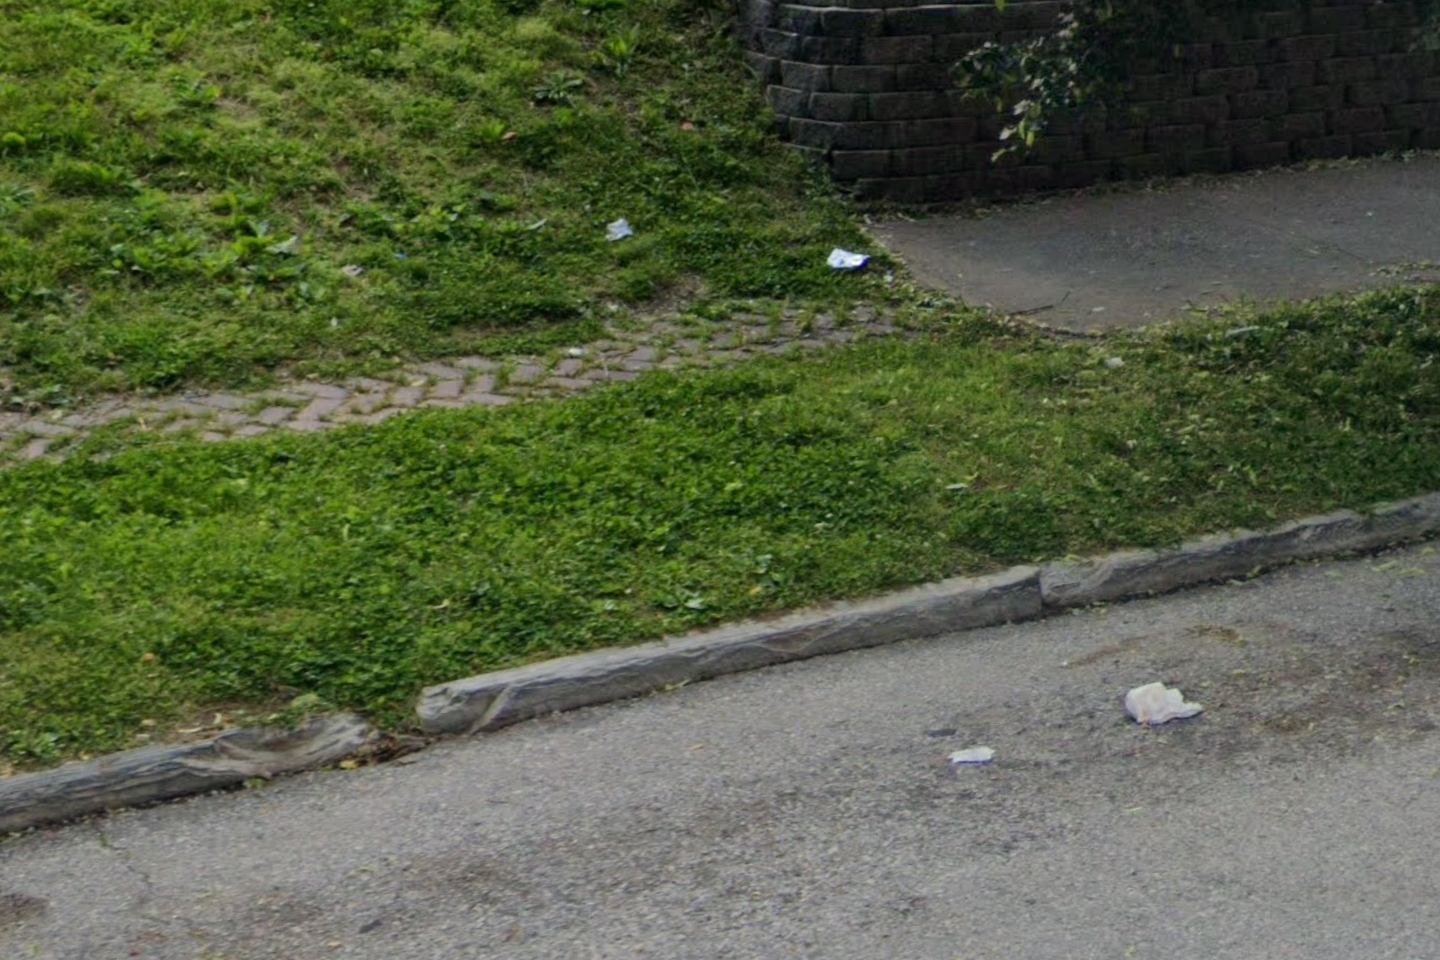
\includegraphics[width=\linewidth,height=3.0cm,keepaspectratio]{images/sidewalk.jpg}
\caption{\textbf{Divergent opinions.} Bumpy stone pavers near a curb cut produce a manual-wheelchair split of 47\%~no, 9\%~unsure, and 44\%~yes, while walking-cane users vote 76\%~yes.}
\label{fig:teaser_a}
\end{subfigure}
\hfill
\begin{subfigure}[t]{0.32\textwidth}
\centering
\vspace{0pt}
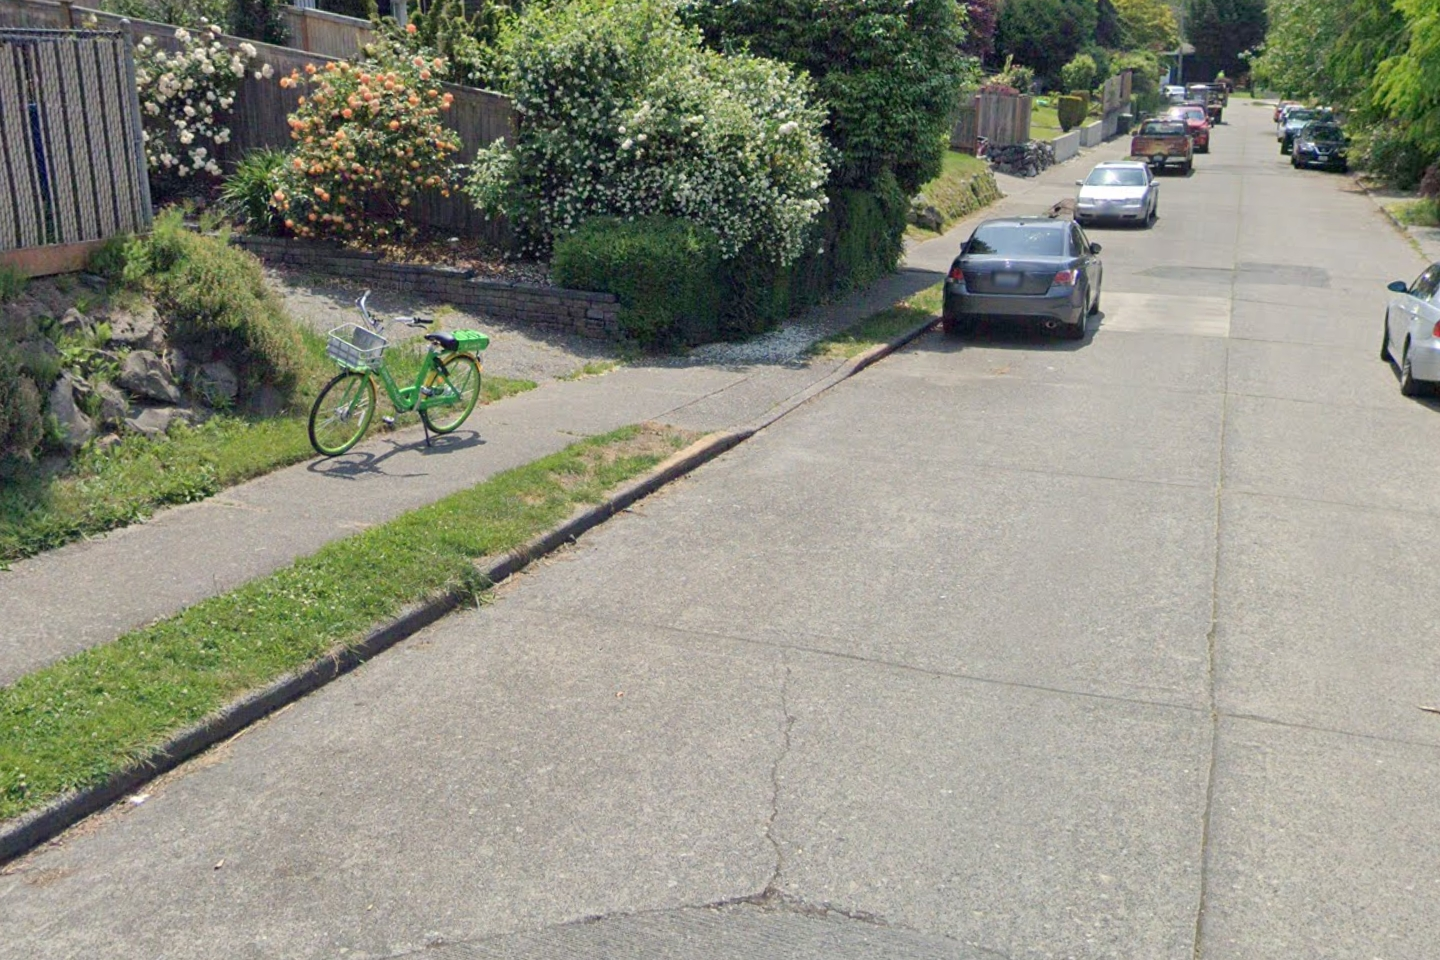
\includegraphics[width=\linewidth,height=3.0cm,keepaspectratio]{images/example2.jpg}
\caption{\textbf{Soft-label perception.} A frozen encoder plus linear probe predicts per-aid distributions $[\hat{p}_\mathrm{no}, \hat{p}_\mathrm{unsure}, \hat{p}_\mathrm{yes}]$ instead of binary classes.}
\label{fig:teaser_b}
\end{subfigure}
\hfill
\begin{subfigure}[t]{0.32\textwidth}
\centering
\vspace{0pt}
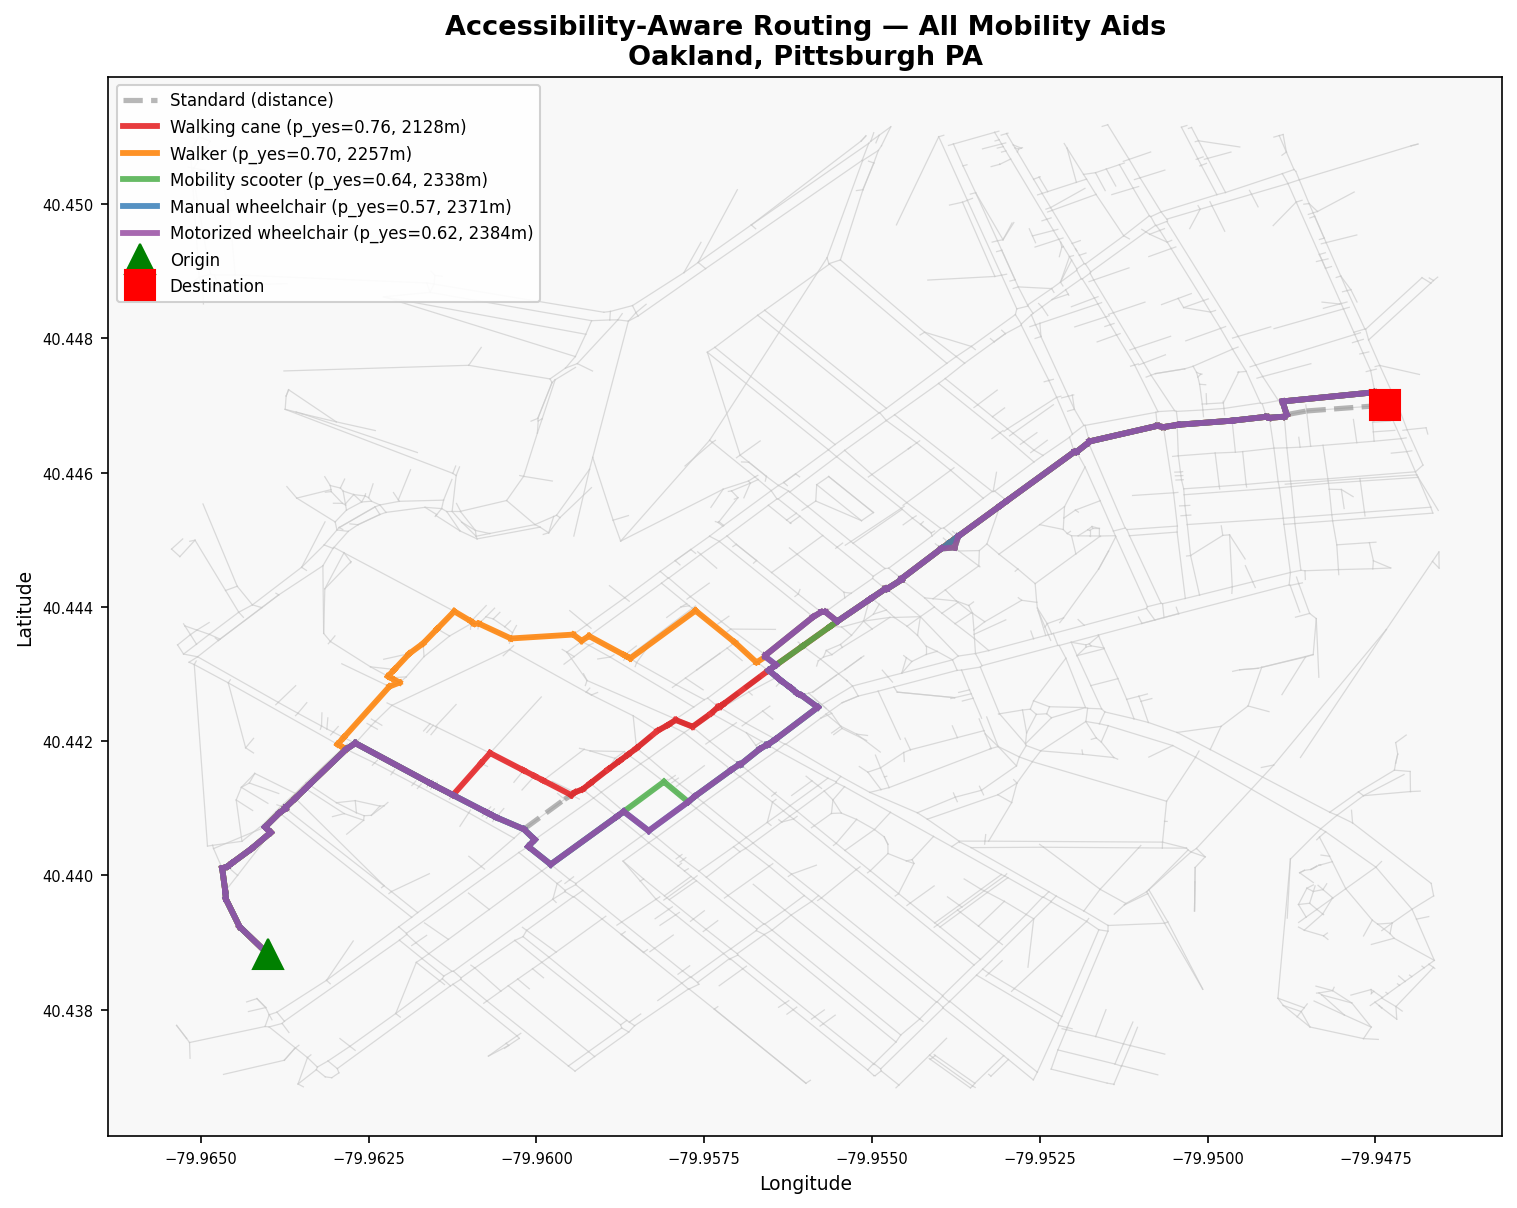
\includegraphics[width=\linewidth,height=3.0cm,keepaspectratio]{images/route_all_aids_overlay.png}
\caption{\textbf{Routing.} Calibrated per-aid edge probabilities in a Pittsburgh graph yield distinct routes per aid and beat OpenRouteService on all five aids.}
\label{fig:teaser_c}
\end{subfigure}
\caption{\textbf{From vote distributions to accessibility-aware routing.} Crowdsourced disagreement is signal, not noise. We train a calibrated per-aid probe from soft labels, embed the resulting probabilities into a pedestrian graph, and demonstrate a routing system that produces a different optimal path for each mobility aid.}
\label{fig:teaser}
\end{figure*}

\section{Related Work}
\label{sec:related}

\textbf{Automated accessibility perception and pedestrian routing.} A decade of work crowdsources sidewalk audits from Street View~\citep{10.1145/2470654.2470744,10.1145/2642918.2647403,10.1145/3308561.3353798,Saha_ProjectSidewalk_CHI2019}, scales them with deep classifiers~\citep{o'meara2025rampnet,10.1145/3663548.3688531}, and complements them with aerial sidewalk extraction~\citep{hosseini2023tile2net,hosseini2022citysurfaces} and multimodal robot/phone sensing~\citep{damaceno2024sideseeing,10.1145/3441852.3476560}. A separate line builds map-level routing engines that consume accessibility metadata: OpenRouteService's wheelchair profile~\citep{openrouteservice2026wheelchair} parses OSM tags into edge costs, AccessMap and the OpenSidewalks schema~\citep{bolten2017accessmap,bolten2019opensidewalks} formalise per-user pedestrian network data, MyPath~\citep{saha2022mypath} adds survey-elicited per-user weights, and Tannert and Sch{\"o}ning~\citep{tannert2018wheelchair} document the tens-of-percent distance penalty wheelchair users pay today. Every prior accessibility classifier trains on hard labels, and every routing engine relies on sparse rule-based OSM tags. We learn a calibrated per-aid probability from \emph{mobility-aid users' own} vote distributions and use it as a drop-in Dijkstra edge cost, covering 91.7\% of edges via direct image inference where ORS-style tag lookup leaves 20\% of OD pairs unroutable.

\textbf{Foundation encoders for robot perception.} CLIP~\citep{radford2021learningtransferablevisualmodels}, DINOv2~\citep{oquab2023dinov2}, and SigLIP2~\citep{tschannen2025siglip2} have become standard backbones for transfer in robot-learning systems where downstream data is scarce. We evaluate all three families plus supervised ViT~\citep{dosovitskiy2021an} on the same folds; the calibration gap between training objectives we report is essentially backbone-invariant.

\textbf{Soft labels and calibration for safety-critical learning.} Label Distribution Learning~\citep{geng2016label} and the CIFAR-10H benchmark~\citep{peterson2019humanuncertainty} established empirical vote distributions as first-class training targets, with subsequent extensions to ImageNet-16H~\citep{steyvers2022bayesian}, sparse-annotator regimes~\citep{collins2022elicit}, crowd-distance selective prediction~\citep{jiang2024crowdcalibrator}, and broad task coverage~\citep{xia2025softlabels}. Soft-label distillation~\citep{hinton2015distilling} is structurally identical but uses a teacher model rather than humans as the source. In parallel, Guo et al.~\citep{guo2017calibration} and Minderer et al.~\citep{minderer2021revisiting} showed that modern networks are systematically overconfident on subjective inputs, and Zollo et al.~\citep{zollo2025calibration} make calibration the primary safety target for embodied agents whose downstream planner consumes probability outputs. Our contribution sits at that intersection: the soft Brier metric is selected by the planner, not by aesthetic preference.

\textbf{Zero-shot VLMs as a perception alternative.} Instruction-tuned VLMs~\citep{liu2023llava,bai2023qwenvl,10.5555/3618408.3619222,chen2024internvl} are increasingly proposed as drop-in perception for robotic tasks. We provide the first latency- and calibration-grounded comparison against trained encoder probes on the accessibility task: even the strongest VLM trails our best probe in calibration by $6\times$ and in latency by $\sim 75\times$.

\section{Dataset and Soft-Label Formulation}
\label{sec:dataset}

\textbf{Data.} Project Sidewalk~\citep{Saha_ProjectSidewalk_CHI2019,DBLP:journals/corr/abs-2502-19888} supplies $49{,}490$ ternary responses (yes/unsure/no) from $829$ mobility-aid users on $52$ rectilinear $640{\times}640$ Google Street View deprojections, $4.4\times$ the CHI 2025 release on the same platform. Each view is rated under each of five aids (manual wheelchair, motorized wheelchair, mobility scooter, walker, walking cane), giving $260$ (image, aid) pairs with $\approx 190$ votes/pair (range 141--240). The $52$ views span nine cities (Amsterdam, CDMX, Chicago, Columbus~OH, La~Piedad~MX, Oradell~NJ, Seattle, St.~Louis, Teaneck~NJ)---none from Pittsburgh, ruling out training-to-routing geographic leakage. The same pixel-identical images are shown to humans and to the model. A YOLOv12-seg~\citep{tian2025yolov12attentioncentricrealtimeobject} area-ratio check $A_{\mathrm{pred}}/A_{\mathrm{gt}}\in[0.7,1.3]$ filters $\sim 60$ candidates to the final $52$; train/test splits are panorama-level at seed $42$. Participants contributed voluntarily via Project Sidewalk's public platform; no personally identifiable information is retained.

\textbf{Vote aggregation and soft labels.} For each pair $(i,a)$ with $K$ votes we form
$\mathbf{y}_{i,a} = K^{-1}\sum_{k} \mathrm{one\_hot}(v_{k,a}) \in \Delta^2$, an empirical distribution over $\{$no, unsure, yes$\}$. Its entropy $H(\mathbf{y}_{i,a}) = -\sum_c y_{i,a}^{(c)} \log y_{i,a}^{(c)}$ defines the sample weight $w_{i,a} = 1 - H(\mathbf{y}_{i,a})/\hmax$ that down-weights highly ambiguous examples during training. Vote entropy is high across all five aids (mean normalised entropy $0.77$--$0.90$; Appendix~\ref{app:dataset}, Fig.~\ref{fig:entropy}), confirming that accessibility is genuinely probabilistic rather than mislabeled.

\textbf{Why a small visual set is appropriate.} The probe (\S\ref{sec:method}) has only $3(d{+}1)$ parameters per aid ($d=1024 \Rightarrow 3075$ for DINOv2-large) and is fit against $52$ vector-valued targets per aid; each target component is the mean of $\sim$60--70 Bernoulli draws (binomial $95\%$ CI $\pm 0.06$--$0.13$). Pixel-level features come from foundation encoders pretrained on $10^8$--$10^9$ images~\citep{radford2021learningtransferablevisualmodels,oquab2023dinov2,tschannen2025siglip2}; the probe learns an aid-conditioned linear projection onto the 3-simplex. The calibration claim is therefore local to the support of these $52$ scenes---we treat the visual sample size as the headline limitation in \S\ref{sec:limitations}. Walking cane shows the strongest yes-skew (45/52 majority-yes, 6.4:1) and motorised wheelchair is evenly split (26/26); the imbalance asymmetry drives the per-aid behaviour analysed in \S\ref{sec:results}.

\FloatBarrier
\section{Method}
\label{sec:method}

\subsection{Linear Probe on Frozen Encoders}

Each image $x_i$ is embedded by a frozen encoder $E$ and L2-normalised: $\mathbf{f}_i = E(x_i)/\|E(x_i)\|_2$. A per-aid linear head produces predictions:
\begin{equation}
\hat{\mathbf{y}}_{i,a} = \mathrm{softmax}(W_a\,\mathbf{f}_i + b_a). \end{equation}
Encoder weights are never updated. We evaluate eight encoders: CLIP ViT-B/32, ViT-B/16, and ViT-L/14~\citep{radford2021learningtransferablevisualmodels}; DINOv2-base and DINOv2-large~\citep{oquab2023dinov2}; SigLIP2-base and SigLIP2-SO400M~\citep{tschannen2025siglip2}; and supervised ViT-B/16 from timm~\citep{dosovitskiy2021an}.

\subsection{Soft-KL Divergence Training}

The primary loss minimises the entropy-weighted KL divergence from model output to human vote distribution:
\begin{equation}
\mathcal{L}_{\mathrm{Soft\text{-}KL}} = \sum_{i,a} w_{i,a}\;\kl\!\bigl(\mathbf{y}_{i,a} \;\|\; \hat{\mathbf{y}}_{i,a}\bigr).
\label{eq:softkl}
\end{equation}
Unlike knowledge distillation, where soft targets come from a teacher model, the targets here are empirical human distributions backed by $\approx 190$ independent judgments each. The predicted $\hat{\mathbf{y}}_{i,a}$ is directly interpretable as ``the fraction of users in our study who would consider this sidewalk accessible.''

\subsection{Hard Cross-Entropy Baseline}

For comparison, we collapse each vote distribution to its argmax label $\hat{c}_{i,a} = \arg\max \mathbf{y}_{i,a}$ and train with standard cross-entropy:
\begin{equation}
\mathcal{L}_{\mathrm{Hard\text{-}CE}} = \sum_{i,a} w_{i,a}\;\mathrm{CE}\!\bigl(\hat{c}_{i,a},\,\hat{\mathbf{y}}_{i,a}\bigr).
\end{equation}
The entropy weight is retained so the comparison isolates the effect of the target (distribution vs.\ hard label) rather than the weighting. As a stronger baseline, we also evaluate post-hoc \textbf{temperature-scaled Hard-CE} (20\% calibration split, NLL objective; Appendix~\ref{app:calibration}).

\subsection{Calibration Metric: Soft Brier Score}

We assess calibration against the human vote distribution:
\begin{equation}
\brier = \frac{1}{N}\sum_{i,a} \bigl\|\hat{\mathbf{y}}_{i,a} - \mathbf{y}_{i,a}\bigr\|_2^2.
\label{eq:brier}
\end{equation}
Lower is better. A model with $\brier = 0.07$ that outputs $\hat{p}_\mathrm{yes} = 0.65$ for a sidewalk where 62\% of users voted ``yes'' is providing actionable probabilistic information. A model with $\brier = 0.23$ outputting $\hat{p}_\mathrm{yes} = 0.97$ for the same image misleads any downstream planner that treats the score as a probability.

\subsection{Training Details}
\label{sec:method:training}

All probes use AdamW (lr $= 10^{-3}$, weight decay $= 10^{-4}$, 50 epochs, batch size 64). Encoder weights are frozen. \textbf{5-fold cross-validation} at the panorama level prevents leakage between rectified crops from the same location. Global seed = 42. All experiments run on a single NVIDIA A100 40 GB GPU. Figure~\ref{fig:pipeline} summarizes the full pipeline; pseudocode for the training loop and the compute/reproducibility details are in Appendix~\ref{app:algo} (Algorithm~\ref{alg:softkl})

\begin{figure*}[!t]
\centering
\resizebox{0.86\textwidth}{!}{%
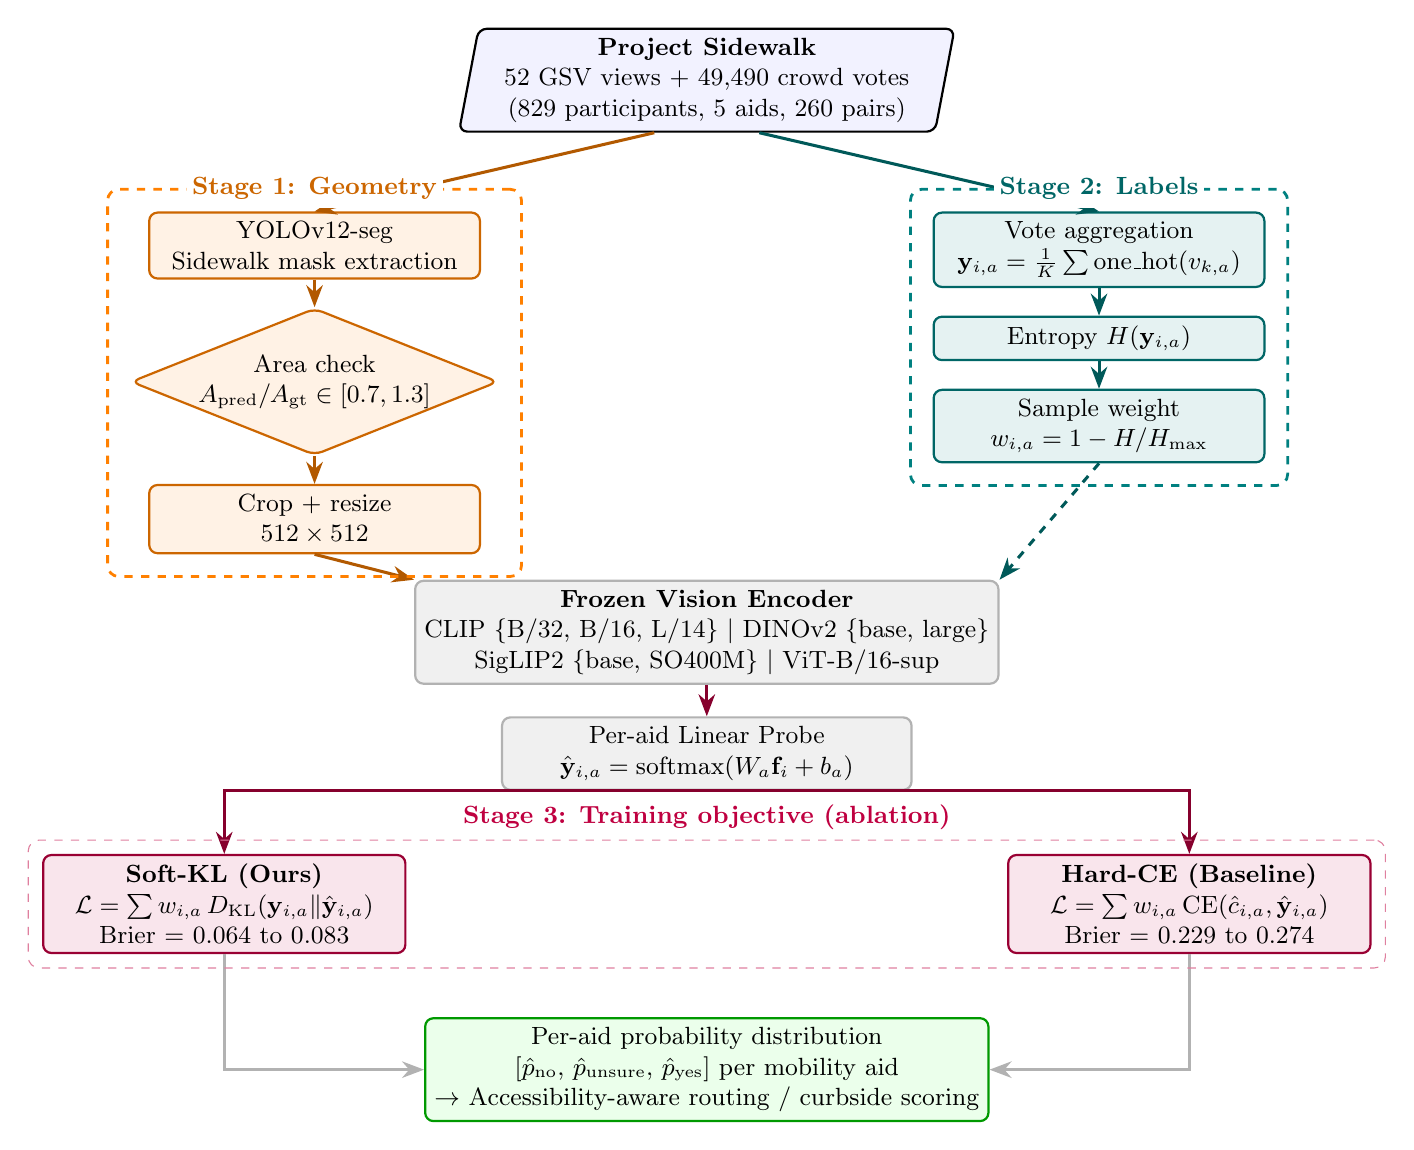
\begin{tikzpicture}[node distance=3.5mm, font=\small, >=Stealth]
\tikzset{
  base/.style={draw, align=center, line width=0.8pt, rounded corners=3pt},
  io/.style={base, fill=blue!5, trapezium, trapezium left angle=80, trapezium right angle=100, trapezium stretches=true, minimum height=0.9cm, minimum width=6.3cm},
  geometry/.style={base, fill=orange!10, draw=orange!80!black, minimum width=4.2cm},
  labels/.style={base, fill=teal!10, draw=teal!80!black, minimum width=4.2cm},
  encoder/.style={base, fill=gray!12, draw=gray!60, minimum width=5.2cm},
  method/.style={base, fill=purple!10, draw=purple!80!black, minimum width=4.6cm},
  output/.style={base, fill=green!8, draw=green!60!black, minimum width=5.5cm},
  arrow/.style={->, thick, draw=gray!60, line width=1.1pt},
  arrow_geo/.style={->, thick, draw=orange!70!black, line width=1.1pt},
  arrow_lab/.style={->, thick, draw=teal!70!black, line width=1.1pt},
  arrow_mod/.style={->, thick, draw=purple!70!black, line width=1.1pt},
}

% Input
\node (data) [io] {\textbf{Project Sidewalk}\\52 GSV views + 49{,}490 crowd votes\\(829 participants, 5 aids, 260 pairs)};

% Stage 1: Geometry
\node (seg) [geometry, below left=10mm and 22mm of data] {YOLOv12-seg\\Sidewalk mask extraction};
\node (verify) [geometry, below=of seg, diamond, aspect=2.5, inner sep=0pt] {Area check\\$A_{\text{pred}}/A_{\text{gt}} \in [0.7,1.3]$};
\node (crop) [geometry, below=of verify] {Crop + resize\\$512 \times 512$};

% Stage 2: Labels
\node (agg) [labels, below right=10mm and 22mm of data] {Vote aggregation\\$\mathbf{y}_{i,a}=\frac{1}{K}\sum \mathrm{one\_hot}(v_{k,a})$};
\node (ent) [labels, below=of agg] {Entropy $H(\mathbf{y}_{i,a})$};
\node (wgt) [labels, below=of ent] {Sample weight\\$w_{i,a}=1-H/H_{\max}$};

% Stage 1 arrows
\draw[arrow_geo] (data.south west) -- (seg.north);
\draw[arrow_geo] (seg) -- (verify);
\draw[arrow_geo] (verify) -- (crop);
\draw[arrow_lab] (data.south east) -- (agg.north);
\draw[arrow_lab] (agg) -- (ent);
\draw[arrow_lab] (ent) -- (wgt);

% Frozen Encoder
\coordinate (branchmid) at ($(crop.south)!0.5!(wgt.south)$);
\node (enc) [encoder, below=9mm of branchmid] {\textbf{Frozen Vision Encoder}\\CLIP \{B/32, B/16, L/14\} $|$ DINOv2 \{base, large\}\\SigLIP2 \{base, SO400M\} $|$ ViT-B/16-sup};
\draw[arrow_geo] (crop.south) -- (enc.north west);
\draw[arrow_lab, dashed] (wgt.south) -- (enc.north east);

% Linear Probe
\node (probe) [encoder, below=4mm of enc] {Per-aid Linear Probe\\$\hat{\mathbf{y}}_{i,a}=\mathrm{softmax}(W_a\mathbf{f}_i+b_a)$};
\draw[arrow_mod] (enc) -- (probe);

% Two training branches
\node (softkl) [method, below left=8mm and 12mm of probe] {\textbf{Soft-KL (Ours)}\\$\mathcal{L}=\sum w_{i,a}\,D_{\mathrm{KL}}(\mathbf{y}_{i,a}\|\hat{\mathbf{y}}_{i,a})$\\Brier = 0.064 to 0.083};
\node (hardce) [method, below right=8mm and 12mm of probe] {\textbf{Hard-CE (Baseline)}\\$\mathcal{L}=\sum w_{i,a}\,\mathrm{CE}(\hat{c}_{i,a},\hat{\mathbf{y}}_{i,a})$\\Brier = 0.229 to 0.274};
\draw[arrow_mod] (probe.south) -| (softkl.north);
\draw[arrow_mod] (probe.south) -| (hardce.north);

% Output
\coordinate (outmid) at ($(softkl.south)!0.5!(hardce.south)$);
\node (out) [output, below=8mm of outmid] {Per-aid probability distribution\\$[\hat{p}_\mathrm{no},\,\hat{p}_\mathrm{unsure},\,\hat{p}_\mathrm{yes}]$ per mobility aid\\$\rightarrow$ Accessibility-aware routing / curbside scoring};
\draw[arrow] (softkl.south) |- (out.west);
\draw[arrow] (hardce.south) |- (out.east);

% Dashed boxes
\node (stagegeom) [draw=orange, dashed, line width=1pt, rounded corners, fit=(seg)(verify)(crop), inner sep=8pt] {};
\node (stagelabels) [draw=teal, dashed, line width=1pt, rounded corners, fit=(agg)(ent)(wgt), inner sep=8pt] {};
\node[orange!80!black, fill=white, inner xsep=2pt, font=\small\bfseries, anchor=center] at (stagegeom.north) {Stage 1: Geometry};
\node[teal!80!black, fill=white, inner xsep=2pt, font=\small\bfseries, anchor=center] at (stagelabels.north) {Stage 2: Labels};
\node[draw=purple!50, dashed, rounded corners, fit=(softkl)(hardce), inner sep=5pt, label={[purple, font=\small]north:\textbf{Stage 3: Training objective (ablation)}}] {};

\end{tikzpicture}%
}
\caption{End-to-end pipeline. Geometry verification (orange) and entropy-weighted soft labels (teal) feed a frozen vision encoder and per-aid probe. Soft-KL preserves calibrated per-aid distributions for routing, while Hard-CE is the collapsed-label baseline.}
\label{fig:pipeline}
\end{figure*}

\section{Results: Calibrated Learned Perception}
\label{sec:results}

All numbers below are 5-fold panorama-level CV at seed $42$; $\pm$ values are 95\% CIs over the $40$ (fold, aid) measurements per encoder. The claim is not visual foundation-model learning but whether frozen urban-scene features can be calibrated against dense human vote distributions to produce a probability a planner can consume.

\textbf{Calibration headline.} Table~\ref{tab:results_all} and Fig.~\ref{fig:brier} (Appendix~\ref{app:calibration}) report the primary calibration result alongside argmax F1. Soft-KL achieves a soft Brier score of $0.064$--$0.083$ versus $0.228$--$0.274$ for Hard-CE---a \textbf{$3.2\times$ mean improvement} consistent across every backbone and outside the 95\% CI for all eight pairings. Post-hoc temperature scaling (NLL-tuned per fold; Appendix~\ref{app:calibration}, Table~\ref{tab:temp_scaling}) reduces Hard-CE Brier by ${\approx}34\%$ on average but leaves a $>2\times$ gap vs Soft-KL, confirming the advantage is structural (target encoding) rather than overconfidence alone. At $\beta_c{=}8$, Hard-CE's overconfident edge probabilities collapse the planner's routing gradient; Soft-KL preserves the empirical bimodality and gives the planner a usable continuous risk signal.

\begin{table}[!t]
\caption{\textbf{Per-encoder results, Soft-KL (ours) vs.\ Hard-CE baseline.} 5-fold panorama-level CV at seed $42$; $\pm$ is 95\% CI over $40$ (fold, aid) measurements. F1 = macro-F1; Brier $\downarrow$ is the soft Brier score against human vote distributions. The bottom block reports zero-shot VLMs evaluated without any task-specific data. The Brier gap is large and consistent across all eight backbones; F1 differences are within their CIs.}
\label{tab:results_all}
\centering\small
\setlength{\tabcolsep}{4pt}
\resizebox{\columnwidth}{!}{%
\begin{tabular}{@{}lcccccc@{}}
\toprule
\textbf{Method} & \textbf{F1 Soft-KL} & \textbf{F1 Hard-CE} & \textbf{Brier Soft-KL} & \textbf{Brier Hard-CE} & \textbf{Ratio} & \textbf{Lat.\ (ms)} \\
\midrule
CLIP B/32      & $0.530\pm0.067$ & $0.617\pm0.059$ & $\mathbf{0.064\pm0.011}$ & $0.231\pm0.016$ & $3.6\times$ &  61.6 \\
CLIP B/16      & $0.499\pm0.060$ & $0.544\pm0.068$ & $0.080\pm0.017$         & $0.239\pm0.025$ & $3.0\times$ &  60.9 \\
CLIP L/14      & $0.531\pm0.065$ & $0.595\pm0.064$ & $0.080\pm0.011$         & $0.230\pm0.022$ & $2.9\times$ &  85.4 \\
DINOv2-base    & $0.496\pm0.064$ & $0.614\pm0.069$ & $0.080\pm0.010$         & $0.238\pm0.024$ & $3.0\times$ &  60.5 \\
DINOv2-large   & $\mathbf{0.613\pm0.071}$ & $0.613\pm0.059$ & $0.075\pm0.013$ & $0.253\pm0.023$ & $3.4\times$ &  78.5 \\
SigLIP2-base   & $0.502\pm0.057$ & $0.596\pm0.060$ & $0.082\pm0.011$         & $\mathbf{0.228\pm0.020}$ & $2.8\times$ &  61.1 \\
SigLIP2-SO400M & $0.579\pm0.064$ & $0.555\pm0.064$ & $0.066\pm0.014$         & $0.256\pm0.022$ & $3.9\times$ & 101.6 \\
ViT-B/16-sup   & $0.482\pm0.073$ & $0.573\pm0.070$ & $0.083\pm0.015$         & $0.274\pm0.027$ & $3.3\times$ &  64.4 \\
\midrule
\textit{Probe mean} & $0.529$    & $\mathbf{0.588}$ & $\mathbf{0.076}$        & $0.244$         & $\mathbf{3.2\times}$ &  -- \\
\midrule
\multicolumn{7}{l}{\textit{Zero-shot VLMs (no task-specific data; F1 / Brier are single-pass)}} \\
Qwen3-VL-8B   & --   & 0.576 & --   & 0.468 & -- & 5{,}919 \\
LLaVA-1.5-7B  & --   & 0.418 & --   & 0.423 & -- &   292 \\
Qwen2.5-VL-7B & --   & 0.412 & --   & 0.632 & -- &   522 \\
\bottomrule
\end{tabular}%
}
\end{table}

\textbf{Why F1 understates the win.} Hard-CE yields higher argmax F1 in six of eight encoders ($+0.059$ on average) but the gap lies inside the 95\% CI in every case. The asymmetry is structural: no image in the dataset has ``unsure'' as the majority vote, so any probability mass Soft-KL faithfully places there is unrecoverable under argmax F1. The encoder ranking also \emph{inverts} between objectives---DINOv2-large leads Soft-KL while CLIP-B/32 leads Hard-CE---indicating that DINOv2's dense self-supervised features better capture the uncertainty structure of human accessibility judgments while CLIP's contrastive language-image features better predict the plurality label.

\textbf{Walking cane: a structural Hard-CE failure preserved by Soft-KL.} Walking cane has a $6.4{:}1$ positive skew ($45/52$ majority-yes). Under Hard-CE, every encoder scores at or below the trivial majority-class baseline of $0.467$, with the best result ($0.513$) only marginally above it; $6/8$ encoders fall \emph{below} the baseline. Soft-KL on DINOv2-large recovers F1 $= 0.640$ ($+42\%$ relative). The mechanism: $5/7$ minority-``no'' walking-cane images have human vote margins $<0.05$ between the top two classes (Appendix~\ref{app:cane}, Fig.~\ref{fig:cane_votes})---near-50/50 splits that Hard-CE coerces into hard negatives, creating contradictory training signal that collapses the model to the majority class. Soft-KL assigns those images targets $\approx[0.45, 0.05, 0.45]$ and preserves the training signal from the two unambiguous ``no'' examples. The robotic-deployment implication is direct: Hard-CE treats near-impassable edges as confidently safe for cane users; Soft-KL flags them as uncertain so the planner routes around them.

\textbf{Zero-shot VLMs trail in both calibration and latency.} The strongest zero-shot VLM (Qwen3-VL-8B) reaches F1 $= 0.576$, within $0.041$ of the best trained probe, but its Brier of $0.468$ is $6.2\times$ worse than DINOv2-large + Soft-KL ($0.075$) and its $5.9$\,s/image latency is $\sim 75\times$ slower than the strongest probe (and $\sim 100\times$ the lightest). LLaVA-1.5 and Qwen2.5-VL collapse to majority-class bias (balanced accuracy near $0.5$). A learned per-aid probe, not a zero-shot prompt, is the configuration a robot planner can consume. Per-prompt sensitivity and the latency Pareto frontier are reported in Appendix~\ref{app:vlm}.

\textbf{Geographic transfer probe.} As an auxiliary encoder-transfer check, distinct from the per-aid task, we evaluate DINOv2-large Soft-KL on binary CurbRamp labels in three unseen cities (Appendix~\ref{app:transfer}, Fig.~\ref{fig:generalization}). Balanced accuracy: Pittsburgh $0.566$ ($n=162$), Detroit $0.570$ ($n=91$), Zurich $0.616$ ($n=89$), Taipei $0.518$ ($n=95$). Pittsburgh/Detroit consistency rules out city-specific overfitting; Zurich gains $+11.6$pp likely because Amsterdam (similar infrastructure) is in the training distribution; Taipei is only $+1.8$pp above chance, a Western-centric-data limit we surface as the constraint on safe deployment (\S\ref{sec:limitations}).

\FloatBarrier
\section{Robot-Planner Interface: Risk-Aware Routing}
\label{sec:routing}

The learned per-aid probability $\hat{p}^a_\mathrm{yes}$ is the perception module's contract with the autonomous-mobility planner. We compose it as an OSM edge cost and show, on a real Pittsburgh pedestrian graph, that risk-aware Dijkstra yields meaningfully different routes per mobility aid and achieves higher model-predicted passability than ORS~\citep{openrouteservice2026wheelchair}. This is an offline planner-facing evaluation: a deployed AV would still verify the immediate curbside scene with onboard sensors before opening the door (Fig.~\ref{fig:teaser}c).

\textbf{Graph and edge scoring.} A fixed Pittsburgh OSM graph ($2{,}046$ nodes, $2{,}618$ undirected edges, single GraphML snapshot) gives the planner topology. We assign per-aid edge priors in three stages: $40.4\%$ of edges match Project Sidewalk GPS labels directly; $51.3\%$ are scored by querying the nearest labeled Street View panorama and running DINOv2-large Soft-KL inference; the remaining $8.3\%$ fall back to population-level priors. Total label-or-image coverage is \textbf{$91.7\%$}. The inferred scores are not constants---mean $\hat{p}_\mathrm{yes}$ across edges ranges from $0.479$ (manual wheelchair) to $0.668$ (walking cane), with $49.5\%$ of manual-wheelchair edges below $0.5$. This spread is precisely what creates a usable routing gradient. The cross-city transfer probe (Appendix~\ref{app:transfer}) is consistent with Pittsburgh GSV being in-distribution against the audit views while Taipei sits outside, matching the transfer-probe limit above.

\textbf{Routing objective and miscalibration cost.} For aid $a$, edge $e$ has cost $\ell_e \cdot (1 + \beta_c\,(1 - \hat{p}^a_{\mathrm{yes},e}))$  (pseudocode in Appendix~\ref{app:algo}, Algorithm~\ref{alg:dijkstra}); we use $\beta_c{=}8$ at the inflection of the Pareto sweep (Appendix~\ref{app:pareto}; $\beta_c\in\{1,2,4,8,16\}$ gives mean $\Delta\bar{p}_\mathrm{yes}$ rising from $0.058$ to $0.105$ at $2.0$--$11.3\%$ distance overhead). Replacing Soft-KL scores with Hard-CE scores at the same $\beta_c$ produces structurally different (and uniformly worse on the calibrated metric) routes for all five aids; Hard-CE \emph{overestimates} its own route's $\hat{p}_\mathrm{yes}$ by $+0.055$ to $+0.085$ because of overconfident edge probabilities. A robot planner consuming Hard-CE outputs would therefore select routes with lower model-predicted passability than Soft-KL alternatives (full breakdown in Appendix~\ref{app:routing_viz}, Table~\ref{tab:supp_crosseval}).

\begin{wraptable}{r}{0.45\textwidth}
\vspace{-10pt}
\caption{\textbf{Canonical OD pair} ($\beta_c{=}8$). Standard-route $\bar{p}_\mathrm{yes}$: $0.442$ (Man.\ WC) to $0.516$ (Cane).}
\label{tab:routing_canonical}
\centering\scriptsize
\setlength{\tabcolsep}{4pt}
\begin{tabular}{@{}lccc@{}}
\toprule
\textbf{Aid} & $\bar{p}^{\mathrm{acc}}_{\mathrm{yes}}$ & $\Delta p_\mathrm{yes}$ & $\Delta\ell$ \\
\midrule
Cane     & 0.671 & +0.155 & +25\% \\
Walker   & 0.630 & +0.144 & +25\% \\
Scooter  & 0.600 & +0.141 & +18\% \\
Man.\ WC & 0.576 & +0.134 & +19\% \\
Mot.\ WC & 0.592 & +0.146 & +25\% \\
\bottomrule
\end{tabular}
\vspace{-8pt}
\end{wraptable}

\textbf{Per-aid routes (canonical OD pair).} Table~\ref{tab:routing_canonical} and Fig.~\ref{fig:teaser}c show the five per-aid paths for one OD pair in the Forbes/Murray corridor: each aid traces a structurally distinct optimal route ($+0.134$ to $+0.155$ mean $\hat{p}_\mathrm{yes}$ at $18$--$25\%$ extra distance). This per-aid diversity is only possible when the planner consumes a real per-edge per-aid probability, not a single binary tag.

\begin{wraptable}{r}{0.50\textwidth}
\vspace{-10pt}
\caption{\textbf{vs.\ ORS} on the 40/50 routable Pittsburgh pairs. Ours yields higher mean $\hat{p}_\mathrm{yes}$ on every aid.}
\label{tab:routing_ors}
\centering\scriptsize
\setlength{\tabcolsep}{4pt}
\begin{tabular}{@{}lccc@{}}
\toprule
\textbf{Aid} & $\bar{p}^{\mathrm{ORS}}_{\mathrm{yes}}$ & $\bar{p}^{\mathrm{ours}}_{\mathrm{yes}}$ & $\Delta$ (95\% CI) \\
\midrule
Cane     & 0.712 & \textbf{0.748} & $+0.036\pm0.018$ \\
Walker   & 0.634 & \textbf{0.668} & $+0.034\pm0.020$ \\
Scooter  & 0.585 & \textbf{0.625} & $+0.040\pm0.019$ \\
Man.\ WC & 0.519 & \textbf{0.566} & $+0.047\pm0.022$ \\
Mot.\ WC & 0.545 & \textbf{0.590} & $+0.045\pm0.022$ \\
\bottomrule
\end{tabular}
\vspace{-8pt}
\end{wraptable}
\textbf{vs.\ OpenRouteService wheelchair profile.} ORS~\citep{openrouteservice2026wheelchair} is the natural rule-based counterpart---it parses OSM wheelchair tags into edge costs and is the engine downstream AccessMap-style products~\citep{bolten2017accessmap,bolten2019opensidewalks,saha2022mypath} would compose with. On 50 random OD pairs in our graph, ORS fails to return a route for $20\%$ of pairs (insufficient OSM tags; a known coverage failure~\citep{tannert2018wheelchair}). On the 40 routable pairs, our learned per-aid scoring yields a higher mean $\hat{p}_\mathrm{yes}$ on every aid (Table~\ref{tab:routing_ors}; full Std/ORS/Ours breakdown in Appendix~\ref{app:routing_viz}, Table~\ref{tab:supp_ors_full}); paired-difference 95\% CIs are positive for all five aids though wide at $n{=}40$, so we read this as directional evidence at one snapshot. The mechanism is coverage: our scoring populates $91.7\%$ of edges with calibrated probabilities, whereas ORS depends on tags absent on most edges of most cities. \emph{Important caveat:} the route-quality comparison ($\Delta\bar{p}_\mathrm{yes}$ in Table~\ref{tab:routing_ors}) uses our model as the scoring function, so it is not fully independent of our optimisation objective; the planner that maximises model-predicted passability will by construction outscore ORS on that same metric. The unambiguously unbiased finding is the $20\%$ ORS coverage failure, which holds regardless of any quality metric and is the primary claim we make about ORS.

\begin{wraptable}{r}{0.52\textwidth}
\vspace{-10pt}
\caption{\textbf{Monte Carlo} over $10{,}000$ random OD pairs ($\beta_c{=}8$, seed 42, min 200\,m). $\pm$ are 95\% Wilson CIs.}
\label{tab:routing_mc}
\centering\scriptsize
\setlength{\tabcolsep}{4pt}
\begin{tabular}{@{}lcccc@{}}
\toprule
\textbf{Aid} & $\overline{\Delta\bar{p}}_\mathrm{yes}$ & Med. & \% impr. & $\overline{\Delta\ell}$ \\
\midrule
Cane     & +0.065 & +0.055 & $87.8\pm0.6$ & +7.4\% \\
Walker   & +0.081 & +0.074 & $88.2\pm0.6$ & +8.2\% \\
Scooter  & +0.102 & +0.096 & $91.0\pm0.6$ & +8.6\% \\
Man.\ WC & +0.120 & +0.112 & $90.9\pm0.6$ & +9.8\% \\
Mot.\ WC & +0.116 & +0.110 & $90.8\pm0.6$ & +9.8\% \\
\bottomrule
\end{tabular}
\vspace{-8pt}
\end{wraptable}
\textbf{Monte Carlo over $10{,}000$ OD pairs.} To verify generality, we sample $10{,}000$ random OD pairs (min separation $200$\,m, seed $42$) and compare standard vs.\ risk-aware Dijkstra (Table~\ref{tab:routing_mc}; the full P25/P50/P75 distribution and per-aid Pareto scatter are reported in Appendix~\ref{app:pareto}). For every aid, $87.8$--$91.0\%$ of trips have higher model-predicted $\hat{p}_\mathrm{yes}$ under risk-aware Dijkstra at $7.4$--$9.8\%$ mean distance overhead; the median overhead is $4.8$--$6.8\%$, indicating most trips reroute at modest cost. This is the behaviour an autonomous mobility planner needs: a hedge that is rarely large in distance but consistently positive in model-predicted passability.


\FloatBarrier
\section{Discussion}
\label{sec:discussion}

\textbf{Calibration is the metric the robot planner selects.} The Dijkstra objective is linear in $\hat{p}_\mathrm{yes}$, so Hard-CE's overconfidence~\citep{guo2017calibration,minderer2021revisiting} directly distorts routing costs. A borderline edge with $62\%$ yes-votes receives $\hat{p}_\mathrm{yes}\approx0.97$ under Hard-CE (penalty $0.24$ at $\beta_c{=}8$) but $\hat{p}_\mathrm{yes}\approx0.65$ under Soft-KL (penalty $2.8$), collapsing the planner's contrast signal across $91.7\%$ of Pittsburgh edges. This is why the model predicts passability gains on $88$--$91\%$ of random OD trips under Soft-KL routing, consistent with calibration-aware deployment guidance for embodied agents~\citep{zollo2025calibration}.

\textbf{Foundation encoders for robot perception.} DINOv2-large leads Soft-KL while CLIP-B/32 leads Hard-CE. The ranking inversion reflects that traversability depends on geometric cues (slope, crack width, surface continuity) where dense self-supervised features outperform language-aligned priors.

\textbf{Hard labels fail under subjective robot-learning signal.} The walking-cane result shows that Hard-CE fails because of target encoding, not encoder choice. For robot-learning tasks based on demonstrations, preferences, or crowd judgments, majority-vote labels can erase the bimodality a downstream planner needs; distribution-valued targets preserve it.

\section{Limitations and Responsible Deployment}
\label{sec:limitations}

\textbf{Visual sample and statistical scope.} Training uses 52 GSV views from nine cities ($3{,}075$ probe parameters per aid for DINOv2-large). The calibration claim rests on the $3.2\times$ Brier ratio between objectives, not absolute F1; encoder rankings within Soft-KL have overlapping CIs (DINOv2-large $0.613{\pm}0.071$ vs.\ SigLIP2-SO400M $0.579{\pm}0.064$) and are suggestive rather than definitive.

\textbf{Geographic and demographic coverage.} Taipei transfer is near chance ($+1.8$\,pp), making Western-centric data the headline limitation. Demographics beyond aid type were not collected, and aid classes conflate equipment geometry, motor power, and individual risk tolerance. A concrete operational rejection criterion: suppress the map-prior in any region where the transfer probe's balanced accuracy is ${\leq}0.55$; Taipei ($0.518$) satisfies this and would be correctly suppressed, while Pittsburgh ($0.566$), Detroit ($0.570$), and Zurich ($0.616$) would be retained. Validating that this threshold generalises requires auditing additional cities, particularly in East Asia and the Global South where our training distribution is absent.

\textbf{Single routing city, offline evaluation, and evaluation circularity.} Routing uses one Pittsburgh OSM snapshot; the ORS comparison is $n{=}50$ pairs and should be read as directional evidence. We have not run a live wheelchair-user study, evaluated transient obstructions or sensor noise, or tested batched/low-power deployment. Critically, the headline routing metric---model-predicted $\hat{p}_\mathrm{yes}$---is the same quantity the risk-aware planner was designed to maximise; the $87.8$--$91.0\%$ improvement therefore demonstrates that the planner successfully optimises its objective, not that the resulting routes are objectively safer for actual users. Verifying the latter would require held-out human audit labels on Pittsburgh edges not seen during training, route-level user-preference studies, or physical traversal measurement with mobility-aid users---none of which we have conducted. As an independent validity check, we correlate model-predicted passability with Project Sidewalk label severity ($1$--$5$ scale) at the edge level (Appendix~\ref{app:ps_val}); severity scores were \emph{never} used in training or routing. On the $188$ graph edges scored via DINOv2-large inference, higher predicted passability is reliably associated with lower nearby PS label severity (Spearman $r{=}0.247$, $p{=}0.0006$), confirming that the learned signal is calibrated against an independent human-annotated accessibility measure. Route-level comparisons (standard vs.\ accessibility-weighted Dijkstra, $40$ OD pairs) show a weaker signal because our detour routes are ${\sim}20\%$ longer, encountering more labels by virtue of covering more ground; the edge-level analysis removes this length confound.

\textbf{Responsible deployment.} The per-aid probability is a community-level prior, not a per-user safety guarantee. A deployed system should use it only for route ranking, verify the curbside scene with onboard sensors~\citep{saha2022mypath}, expose uncertainty rather than an argmax, and reject regions where the transfer probe is near chance.

\section{Conclusion}
\label{sec:conclusion}

We presented a learned perception module that treats vote distributions from 829 mobility-aid users as first-class training targets and produces calibrated per-aid passability probabilities for autonomous mobility planning. A frozen-encoder probe trained by KL divergence achieves a $3.2\times$ soft-Brier improvement over hard cross-entropy across eight backbones; composed into risk-aware Dijkstra, it achieves model-predicted passability gains on $87.8$--$91.0\%$ of $10{,}000$ Pittsburgh OD pairs at $7.4$--$9.8\%$ distance overhead and yields higher model-predicted passability than OpenRouteService's wheelchair profile on every tested aid. The central lesson is that when subjective human judgment supervises a downstream policy, calibration---not argmax accuracy---is the operative metric. A natural extension is to fine-tune VLMs with Soft-KL versus Hard-CE targets (via LoRA on the same 52-image folds), testing whether the structural advantage of distribution-valued training targets observed in linear probes extends to billion-parameter backbones—and whether soft labels close the $6\times$ Brier gap even when the backbone itself is far more expressive. Code and pre-extracted features will be released upon acceptance.

% Bibliography style (corlabbrvnat) is set by the corl_2026 package.
\bibliography{refs}

% ============================================================
% APPENDICES
% ============================================================
\clearpage
\appendix
\makeatletter
\@addtoreset{table}{section}
\@addtoreset{figure}{section}
\makeatother
\renewcommand{\thesection}{\Alph{section}}
\renewcommand{\thetable}{\thesection.\arabic{table}}
\renewcommand{\thefigure}{\thesection.\arabic{figure}}
\setcounter{section}{0}
\setcounter{table}{0}
\setcounter{figure}{0}

% Liberalize float placement so multiple tables/figures can share a page
% with body text instead of being pushed onto a float-only page.
\setcounter{topnumber}{4}
\setcounter{bottomnumber}{2}
\setcounter{totalnumber}{6}
\renewcommand{\topfraction}{0.95}
\renewcommand{\bottomfraction}{0.95}
\renewcommand{\textfraction}{0.05}
\renewcommand{\floatpagefraction}{0.7}

\noindent\emph{The appendices report the full per-encoder, per-aid, and per-OD-pair breakdowns that support the headline numbers in the main paper. Tables, figures, and equations are numbered with the prefix of their parent appendix section (e.g., Fig.~A.1, Table~B.3).}

\section{Dataset and Annotator Disagreement}
\label{app:dataset}

This appendix details the annotator-vote distributions that motivate our soft-label training: per-pair entropy across all five mobility aids, and representative Project Sidewalk audit views illustrating per-aid disagreement.

\begin{figure}[!ht]
\centering
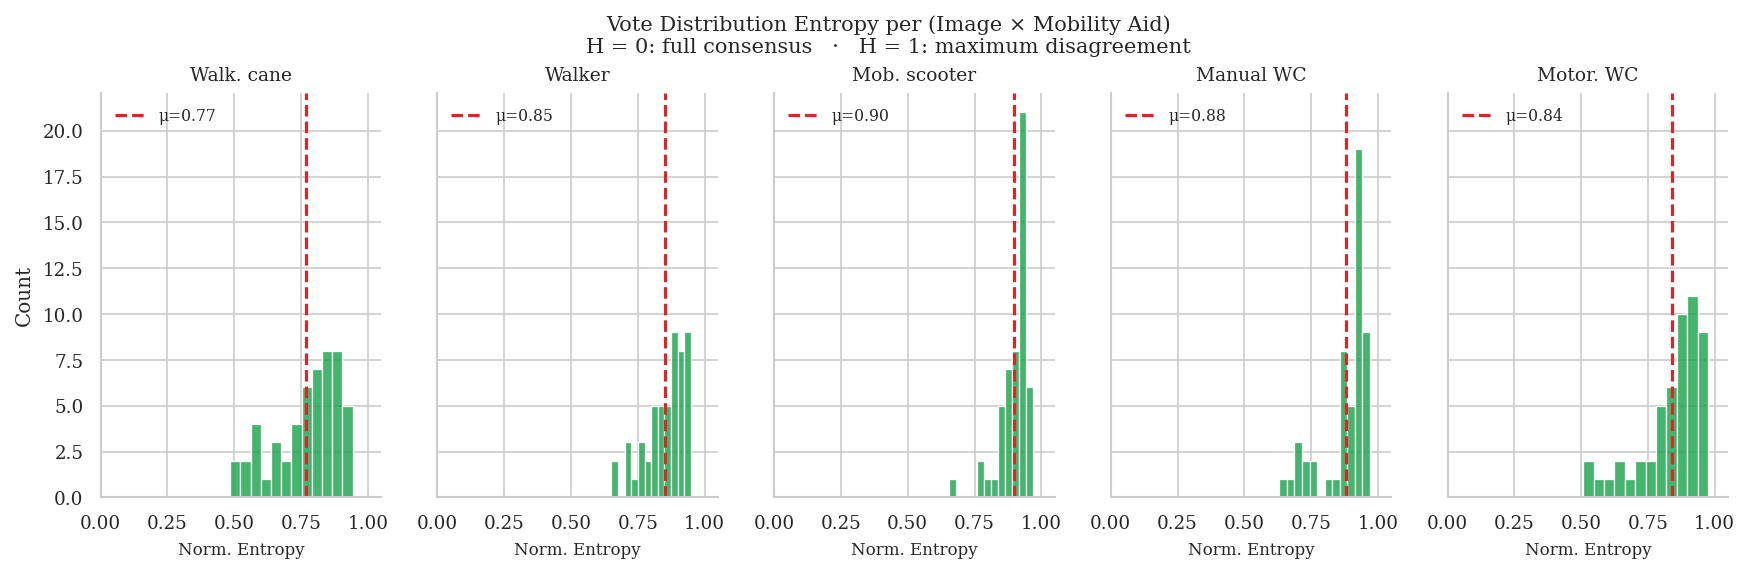
\includegraphics[width=0.85\linewidth]{images/fig5_entropy_histogram.png}
\caption{Normalised vote entropy per (image, aid) pair for all five mobility aids. Dashed red line = per-aid mean. Consistently high entropy across all aids confirms that soft-label training is warranted and that hard majority labels discard genuine information.}
\label{fig:entropy}
\end{figure}

\begin{figure}[!ht]
\centering
\begin{subfigure}[t]{0.48\linewidth}
\centering
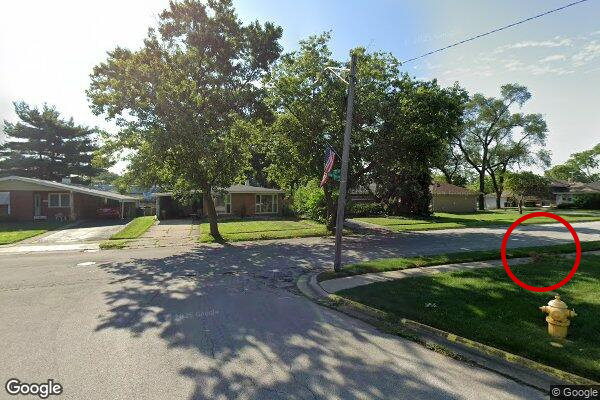
\includegraphics[width=\linewidth,height=2.8cm,keepaspectratio]{images/View1_Circle.jpg}
\caption{Sparse cue: missing curb ramp at intersection. Manual WC ``no'' $= 78\%$.}
\end{subfigure}
\hfill
\begin{subfigure}[t]{0.48\linewidth}
\centering
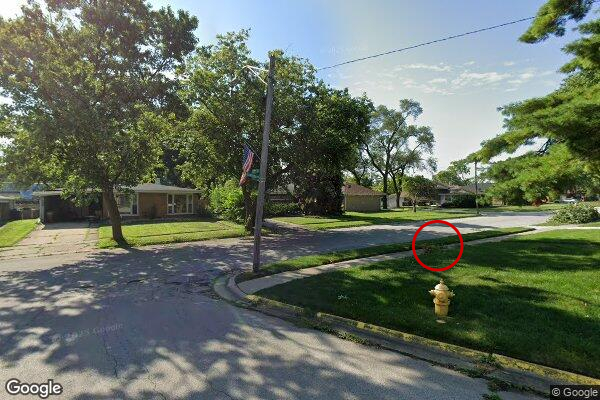
\includegraphics[width=\linewidth,height=2.8cm,keepaspectratio]{images/View2_Circle.jpg}
\caption{Similar scene, but the lawn-strip transition is passable. Manual WC ``yes'' $= 61\%$.}
\end{subfigure}\\[0.4em]
\begin{subfigure}[t]{0.48\linewidth}
\centering
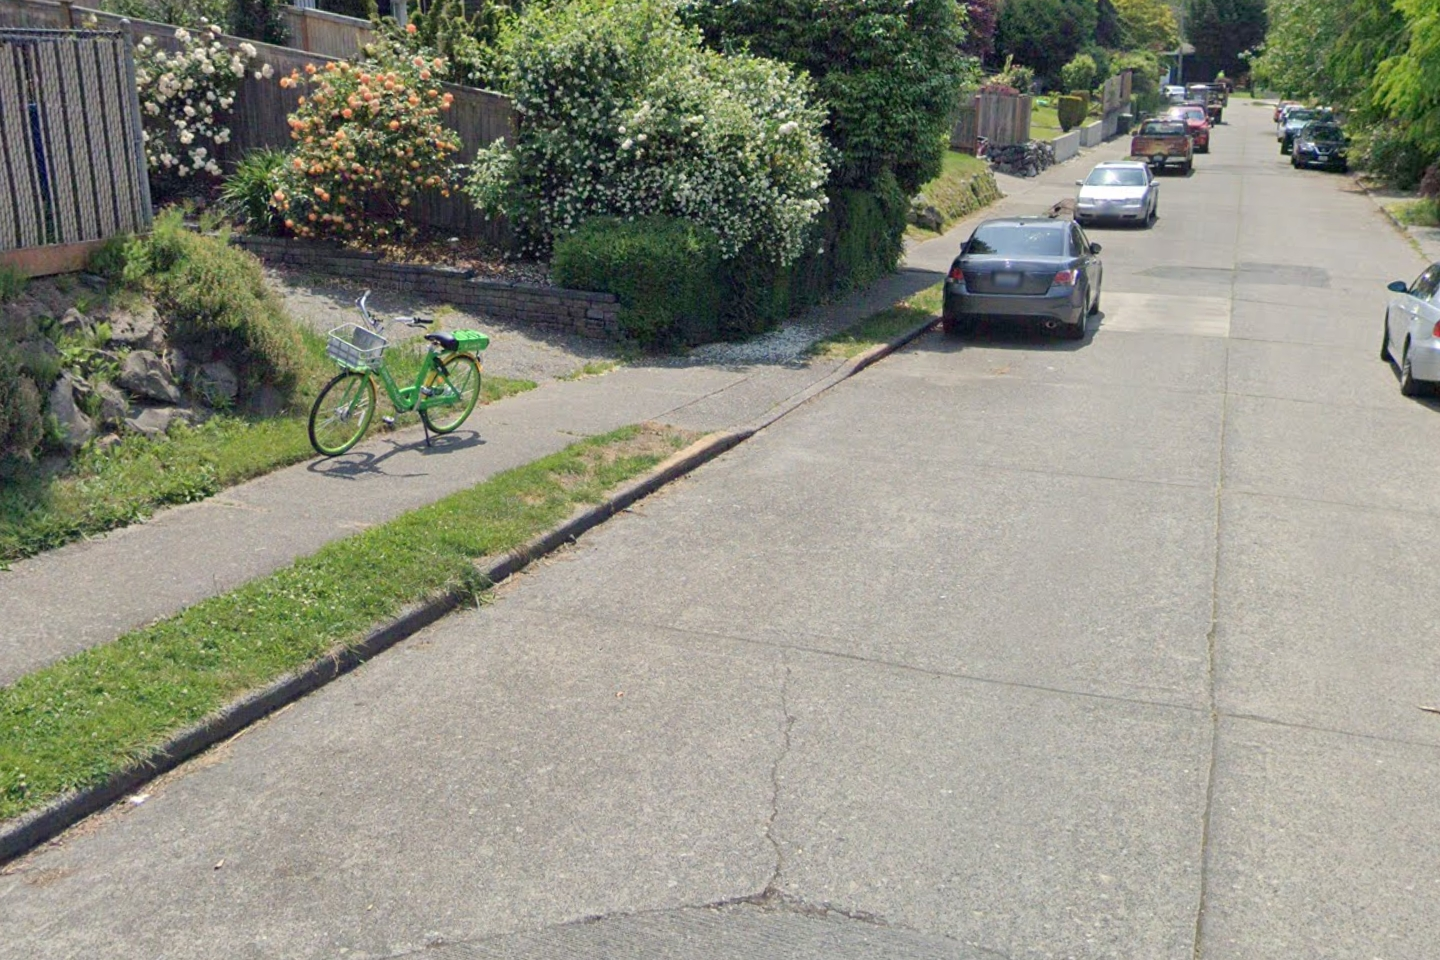
\includegraphics[width=\linewidth,height=2.8cm,keepaspectratio]{images/example2.jpg}
\caption{Clean continuous concrete; high inter-aid agreement on ``yes.''}
\end{subfigure}
\hfill
\begin{subfigure}[t]{0.48\linewidth}
\centering
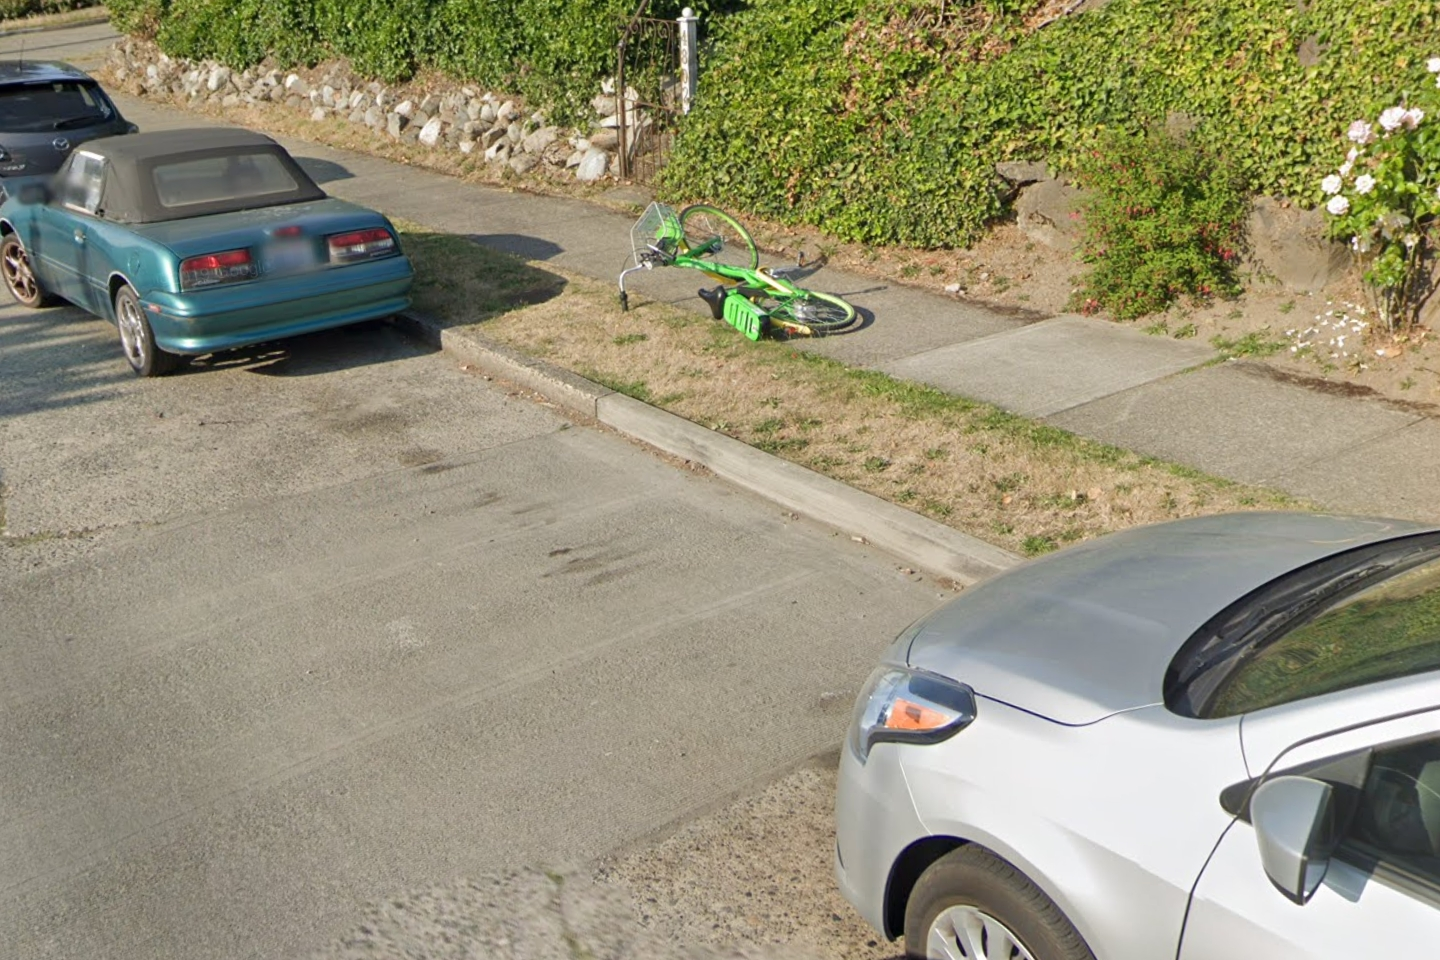
\includegraphics[width=\linewidth,height=2.8cm,keepaspectratio]{images/example3.jpg}
\caption{Driveway obstruction. Manual WC ``no'' $= 56\%$, cane ``yes'' $= 64\%$.}
\end{subfigure}
\caption{Representative Project Sidewalk audit views illustrating per-aid disagreement. Red circles mark the focal region. Adjacent panoramas with near-identical global appearance can produce sharply different per-aid vote distributions.}
\label{fig:sidewalk_examples}
\end{figure}

\FloatBarrier
\section{Full Per-Encoder Per-Aid Calibration Results}
\label{app:calibration}

This appendix expands Table~\ref{tab:results_all} by reporting per-aid macro-F1, soft Brier, and Expected Calibration Error (ECE) for every encoder under both training objectives. All numbers are 5-fold panorama-level CV at seed = 42, identical to the main paper. Bold cells highlight the best encoder per aid within each objective. Figs.~\ref{fig:heatmap} and~\ref{fig:brier} visualise the same data. Table~\ref{tab:temp_scaling} additionally reports the effect of post-hoc temperature scaling on Hard-CE.

\begin{figure}[!ht]
\centering
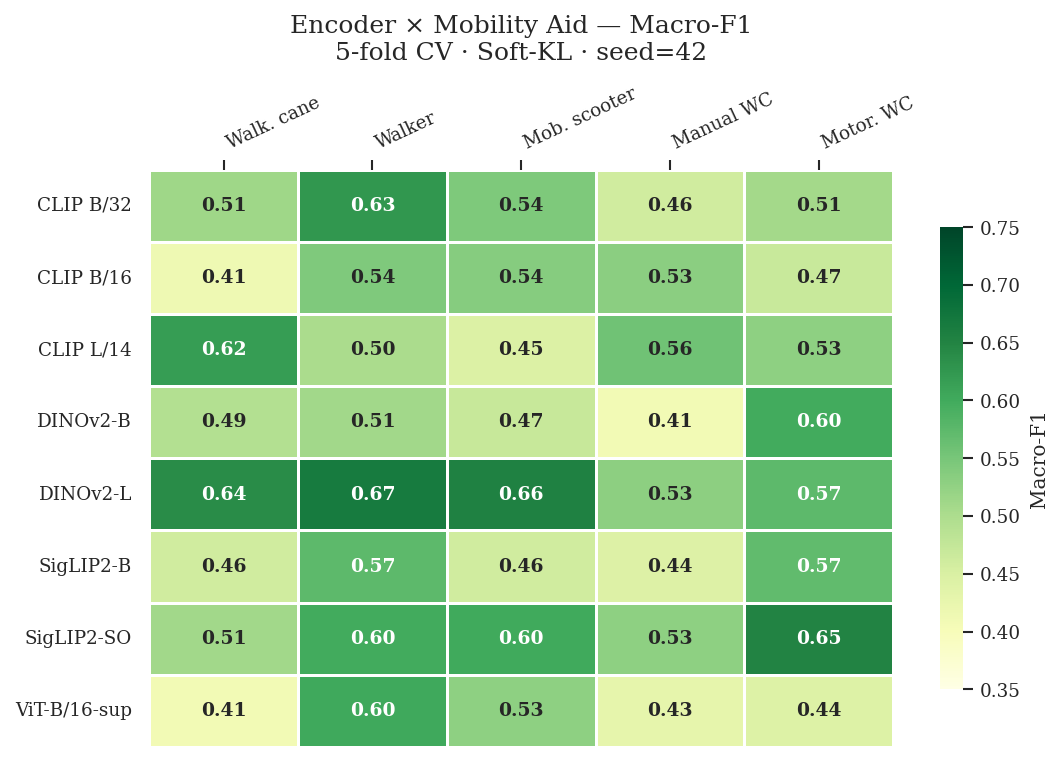
\includegraphics[width=0.85\linewidth]{images/fig1_encoder_f1_heatmap.png}
\caption{Encoder $\times$ mobility aid macro-F1 heatmap under Soft-KL. DINOv2-large shows the most consistent per-aid coverage; walking cane is the hardest aid for every encoder, reflecting its $6.4{:}1$ yes-to-no imbalance.}
\label{fig:heatmap}
\end{figure}

\begin{figure}[!ht]
\centering
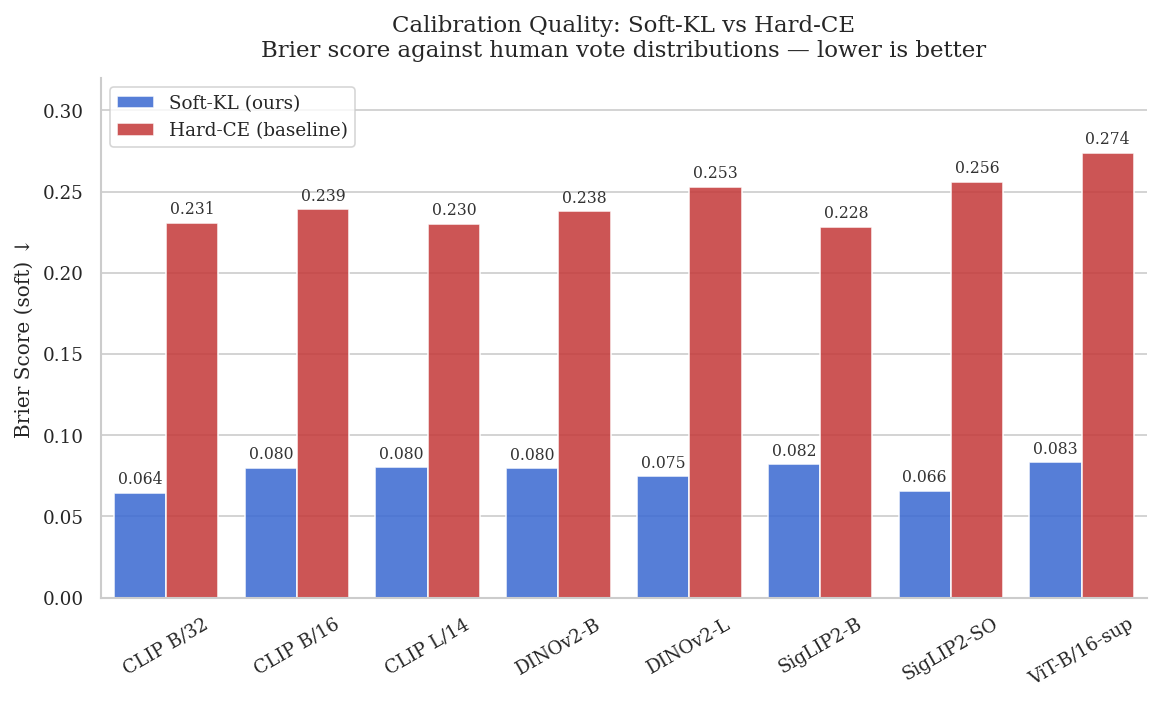
\includegraphics[width=0.85\linewidth]{images/fig2_brier_comparison.png}
\caption{Soft Brier score per encoder: Soft-KL (blue) vs.\ Hard-CE (red). Lower is better. The $\sim 3\times$ gap is consistent across all eight encoders; Hard-CE produces overconfident predictions that misrepresent genuine human uncertainty.}
\label{fig:brier}
\end{figure}

\begin{table}[!ht]
\caption{\textbf{Soft-KL: per-aid macro-F1.} Best per column in bold.}
\label{tab:supp_softkl_f1}
\centering\scriptsize
\setlength{\tabcolsep}{4pt}
\begin{tabular}{@{}lcccccc@{}}
\toprule
\textbf{Encoder} & \textbf{Cane} & \textbf{Walker} & \textbf{Scooter} & \textbf{Man.WC} & \textbf{Mot.WC} & \textbf{Mean} \\
\midrule
CLIP B/32      & 0.513 & 0.625 & 0.544 & 0.459 & 0.509 & 0.530 \\
CLIP B/16      & 0.414 & 0.542 & 0.537 & 0.532 & 0.469 & 0.499 \\
CLIP L/14      & 0.618 & 0.503 & 0.446 & \textbf{0.557} & 0.529 & 0.531 \\
DINOv2-base    & 0.493 & 0.510 & 0.470 & 0.408 & 0.599 & 0.496 \\
DINOv2-large   & \textbf{0.640} & \textbf{0.667} & \textbf{0.656} & 0.531 & 0.573 & \textbf{0.613} \\
SigLIP2-base   & 0.461 & 0.574 & 0.459 & 0.444 & 0.571 & 0.502 \\
SigLIP2-SO400M & 0.511 & 0.600 & 0.601 & 0.530 & \textbf{0.652} & 0.579 \\
ViT-B/16-sup   & 0.408 & 0.603 & 0.529 & 0.429 & 0.442 & 0.482 \\
\bottomrule
\end{tabular}
\end{table}

\begin{table}[!ht]
\caption{\textbf{Hard-CE: per-aid macro-F1.} Best per column in bold.}
\label{tab:supp_hardce_f1}
\centering\scriptsize
\setlength{\tabcolsep}{4pt}
\begin{tabular}{@{}lcccccc@{}}
\toprule
\textbf{Encoder} & \textbf{Cane} & \textbf{Walker} & \textbf{Scooter} & \textbf{Man.WC} & \textbf{Mot.WC} & \textbf{Mean} \\
\midrule
CLIP B/32      & 0.453 & \textbf{0.761} & 0.558 & \textbf{0.675} & 0.639 & \textbf{0.617} \\
CLIP B/16      & 0.434 & 0.536 & 0.569 & 0.562 & 0.618 & 0.544 \\
CLIP L/14      & 0.453 & 0.707 & 0.698 & 0.523 & 0.597 & 0.595 \\
DINOv2-base    & 0.446 & 0.720 & 0.668 & 0.574 & \textbf{0.664} & 0.614 \\
DINOv2-large   & 0.489 & 0.675 & \textbf{0.746} & 0.502 & 0.652 & 0.613 \\
SigLIP2-base   & 0.458 & 0.700 & 0.587 & 0.572 & 0.664 & 0.596 \\
SigLIP2-SO400M & 0.453 & 0.669 & 0.519 & 0.483 & 0.652 & 0.555 \\
ViT-B/16-sup   & \textbf{0.513} & 0.682 & 0.606 & 0.553 & 0.509 & 0.573 \\
\bottomrule
\end{tabular}
\end{table}

\begin{table}[!ht]
\caption{\textbf{Soft-KL: per-aid soft Brier score ($\downarrow$).} Lower is better (perfect calibration = 0). All values $<0.15$, vs.\ Hard-CE values $\geq 0.19$ in Table~\ref{tab:supp_hardce_brier}.}
\label{tab:supp_softkl_brier}
\centering\scriptsize
\setlength{\tabcolsep}{4pt}
\begin{tabular}{@{}lcccccc@{}}
\toprule
\textbf{Encoder} & \textbf{Cane} & \textbf{Walker} & \textbf{Scooter} & \textbf{Man.WC} & \textbf{Mot.WC} & \textbf{Mean} \\
\midrule
CLIP B/32      & 0.051 & 0.066 & 0.044 & 0.059 & 0.103 & 0.064 \\
CLIP B/16      & 0.059 & 0.085 & 0.048 & 0.070 & 0.139 & 0.080 \\
CLIP L/14      & 0.061 & 0.076 & 0.068 & 0.087 & 0.109 & 0.080 \\
DINOv2-base    & 0.072 & 0.079 & 0.063 & 0.082 & 0.102 & 0.080 \\
DINOv2-large   & 0.061 & 0.070 & 0.051 & 0.086 & 0.106 & 0.075 \\
SigLIP2-base   & 0.079 & 0.082 & 0.057 & 0.089 & 0.104 & 0.082 \\
SigLIP2-SO400M & 0.062 & 0.069 & 0.047 & 0.061 & 0.090 & 0.066 \\
ViT-B/16-sup   & 0.065 & 0.082 & 0.061 & 0.075 & 0.133 & 0.083 \\
\bottomrule
\end{tabular}
\end{table}

\begin{table}[!ht]
\caption{\textbf{Hard-CE: per-aid soft Brier score ($\downarrow$).} Uniformly 3 to $4\times$ worse than Soft-KL across all (encoder, aid) cells.}
\label{tab:supp_hardce_brier}
\centering\scriptsize
\setlength{\tabcolsep}{4pt}
\begin{tabular}{@{}lcccccc@{}}
\toprule
\textbf{Encoder} & \textbf{Cane} & \textbf{Walker} & \textbf{Scooter} & \textbf{Man.WC} & \textbf{Mot.WC} & \textbf{Mean} \\
\midrule
CLIP B/32      & 0.229 & 0.213 & 0.234 & 0.243 & 0.234 & 0.231 \\
CLIP B/16      & 0.212 & 0.253 & 0.205 & 0.245 & 0.280 & 0.239 \\
CLIP L/14      & 0.200 & 0.221 & 0.239 & 0.249 & 0.240 & 0.230 \\
DINOv2-base    & 0.195 & 0.208 & 0.265 & 0.291 & 0.230 & 0.238 \\
DINOv2-large   & 0.211 & 0.235 & 0.242 & 0.304 & 0.272 & 0.253 \\
SigLIP2-base   & 0.197 & 0.231 & 0.245 & 0.235 & 0.234 & 0.228 \\
SigLIP2-SO400M & 0.208 & 0.265 & 0.244 & 0.270 & 0.293 & 0.256 \\
ViT-B/16-sup   & 0.218 & 0.288 & 0.268 & 0.259 & 0.336 & 0.274 \\
\bottomrule
\end{tabular}
\end{table}

\begin{table}[!ht]
\caption{\textbf{Expected Calibration Error (ECE, $\downarrow$).} For Manual~WC, Soft-KL achieves lower ECE in 7/8 cases; for Walking Cane the pattern inverts---Soft-KL has higher ECE in all 8 (see note below). Brier score, which penalises probability magnitude rather than just rank, is the operative calibration metric for the planner (cf.\ Tables~\ref{tab:supp_softkl_brier} and~\ref{tab:supp_hardce_brier}).}
\label{tab:supp_ece}
\centering\scriptsize
\setlength{\tabcolsep}{4pt}
\begin{tabular}{@{}lcc|cc@{}}
\toprule
& \multicolumn{2}{c|}{\textbf{Walking cane}} & \multicolumn{2}{c}{\textbf{Manual WC}} \\
\textbf{Encoder} & \textbf{Soft-KL} & \textbf{Hard-CE} & \textbf{Soft-KL} & \textbf{Hard-CE} \\
\midrule
CLIP B/32      & 0.270 & 0.179 & 0.202 & 0.238 \\
CLIP B/16      & 0.275 & 0.205 & 0.214 & 0.219 \\
CLIP L/14      & 0.223 & 0.166 & 0.258 & 0.269 \\
DINOv2-base    & 0.234 & 0.165 & 0.210 & 0.250 \\
DINOv2-large   & 0.243 & 0.185 & 0.274 & 0.303 \\
SigLIP2-base   & 0.193 & 0.192 & 0.262 & 0.225 \\
SigLIP2-SO400M & 0.277 & 0.183 & 0.239 & 0.272 \\
ViT-B/16-sup   & 0.209 & 0.194 & 0.262 & 0.291 \\
\bottomrule
\end{tabular}
\end{table}

\noindent\textbf{Why does Soft-KL have higher ECE for Walking Cane?} ECE measures whether the model's max-confidence matches its argmax accuracy. For Walking Cane (45/52 majority-yes), Hard-CE collapses every prediction to high-confidence ``yes,'' achieving low ECE but missing the minority ``no'' images entirely. Soft-KL deliberately spreads probability mass across classes to match the human vote distribution, which lowers max-confidence and \emph{raises} ECE even as it dramatically improves soft Brier and macro-F1. The planner uses $\hat{p}_\mathrm{yes}$ as an edge cost---not the argmax---so the operative calibration metric is Brier, not ECE.

\begin{table}[!ht]
\caption{\textbf{Temperature-scaled Hard-CE vs.\ Hard-CE and Soft-KL (soft Brier $\downarrow$).}
  For each fold we hold out $20\%$ of training panoramas as a calibration split, minimise NLL over a scalar temperature $T$, and apply the scaled probe to the test fold. Temperature scaling reduces Hard-CE Brier by ${\approx}34\%$ on average, but Soft-KL remains $>2\times$ better across all encoders, confirming that the gain from soft-label training is structural rather than a consequence of overconfidence alone.}
\label{tab:temp_scaling}
\centering\scriptsize
\setlength{\tabcolsep}{5pt}
\begin{tabular}{@{}lcccc@{}}
\toprule
\textbf{Encoder} & \textbf{Soft-KL} & \textbf{Hard-CE} & \textbf{Hard-CE+TS} & \textbf{Mean $T$} \\
\midrule
CLIP B/32        & \textbf{0.064} & 0.231 & 0.147 & 2.04 \\
CLIP B/16        & \textbf{0.080} & 0.239 & 0.186 & 1.84 \\
CLIP L/14        & \textbf{0.080} & 0.230 & 0.156 & 2.48 \\
DINOv2-base      & \textbf{0.080} & 0.238 & 0.172 & 1.98 \\
DINOv2-large     & \textbf{0.075} & 0.253 & 0.151 & 2.42 \\
SigLIP2-base     & \textbf{0.082} & 0.228 & 0.170 & 2.19 \\
SigLIP2-SO400M   & \textbf{0.066} & 0.256 & 0.154 & 2.75 \\
ViT-B/16-sup     & \textbf{0.083} & 0.274 & 0.155 & 2.31 \\
\midrule
\textit{Mean}    & \textbf{0.076} & 0.244 & 0.161 & 2.25 \\
\bottomrule
\end{tabular}
\end{table}

\FloatBarrier
\section{Zero-Shot VLM Analysis}
\label{app:vlm}

This appendix expands the zero-shot VLM bottom block of Table~\ref{tab:results_all} with the inference-latency Pareto frontier (Fig.~\ref{fig:latency}), an aggregated F1 comparison (Fig.~\ref{fig:zeroshot}), and full per-prompt sensitivity across three VLMs (Table~\ref{tab:supp_prompts_full}).

\begin{figure}[!ht]
\centering
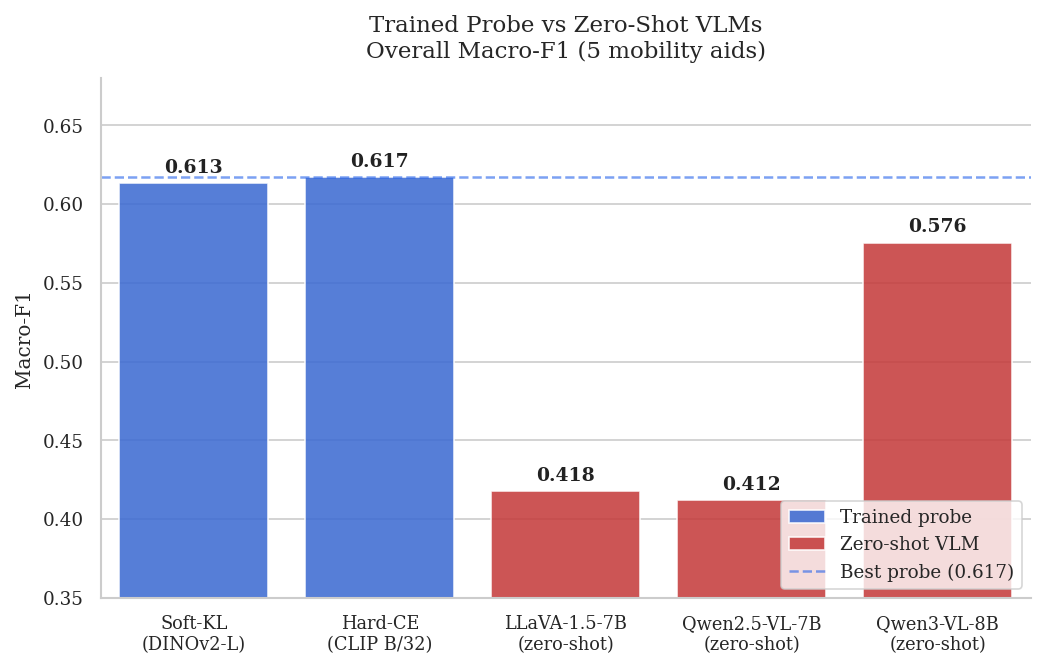
\includegraphics[width=0.70\linewidth]{images/fig4_zeroshot_vs_probe.png}
\caption{Trained probes vs.\ zero-shot VLMs on overall macro-F1. Dashed blue line = best probe (F1 $= 0.617$). Qwen3-VL-8B (F1 $= 0.576$) comes within $0.041$ F1 at $\sim 75\times$ higher latency and $6.2\times$ worse Brier.}
\label{fig:zeroshot}
\end{figure}

\begin{figure}[!ht]
\centering
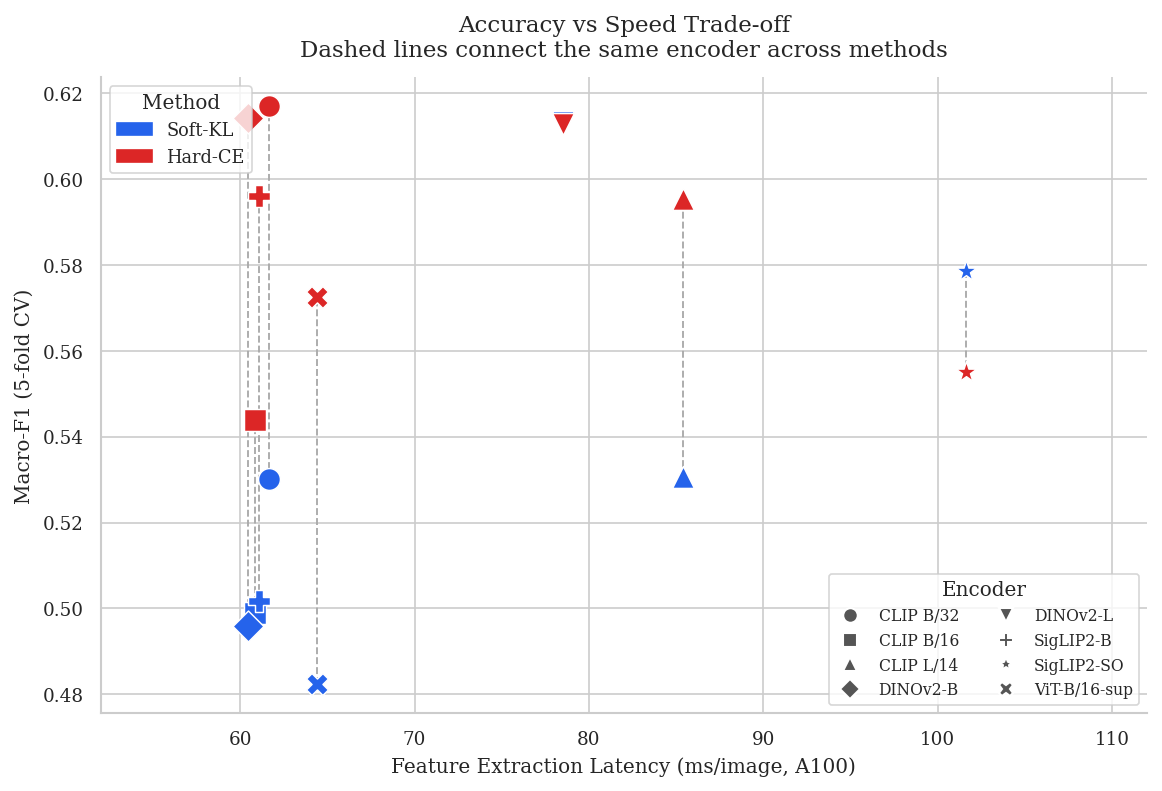
\includegraphics[width=0.75\linewidth]{images/fig3_latency_vs_f1.png}
\caption{Macro-F1 vs.\ inference latency for all 8 encoders under Soft-KL (blue) and Hard-CE (red). DINOv2-large is Pareto-optimal under Soft-KL ($78.5$\,ms, F1 $= 0.613$). All encoder probes fit a real-time routing budget.}
\label{fig:latency}
\end{figure}

\begin{table}[!ht]
\caption{\textbf{Full prompt-sensitivity matrix.} Three prompts (Direct / Descriptive / CoT) $\times$ three VLMs. Best per model in bold. Parse failures = number of responses (out of 260) lacking a parseable ternary label. Only CoT on Qwen2.5-VL-7B incurred any parse failures (2/260), confirming that prompt-engineering effects do not reduce to format-compliance differences.}
\label{tab:supp_prompts_full}
\centering\scriptsize
\setlength{\tabcolsep}{6pt}
\begin{tabular}{@{}llccc@{}}
\toprule
\textbf{Model} & \textbf{Variant} & \textbf{F1} & \textbf{Bal.Acc} & \textbf{Parse fail} \\
\midrule
\multirow{3}{*}{Qwen3-VL-8B}   & Direct      & 0.513 & 0.532 & 0 \\
                                & \textbf{Descriptive} & \textbf{0.576} & \textbf{0.633} & 0 \\
                                & CoT         & 0.547 & 0.563 & 0 \\
\midrule
\multirow{3}{*}{LLaVA-1.5-7B}  & Direct      & 0.488 & 0.520 & 0 \\
                                & Descriptive & 0.430 & 0.514 & 0 \\
                                & \textbf{CoT}         & \textbf{0.542} & \textbf{0.563} & 0 \\
\midrule
\multirow{3}{*}{Qwen2.5-VL-7B} & \textbf{Direct}      & \textbf{0.442} & 0.610 & 0 \\
                                & Descriptive & 0.412 & 0.596 & 0 \\
                                & CoT         & 0.479 & \textbf{0.622} & 2 \\
\bottomrule
\end{tabular}
\end{table}

\FloatBarrier
\section{Walking-Cane Failure Cases}
\label{app:cane}

This appendix supports the walking-cane failure analysis in \S\ref{sec:results}. Figure~\ref{fig:cane_votes} shows the full vote distributions for the seven majority-``no'' walking-cane images that drive the Hard-CE collapse described in the main paper.

\begin{figure}[!ht]
\centering
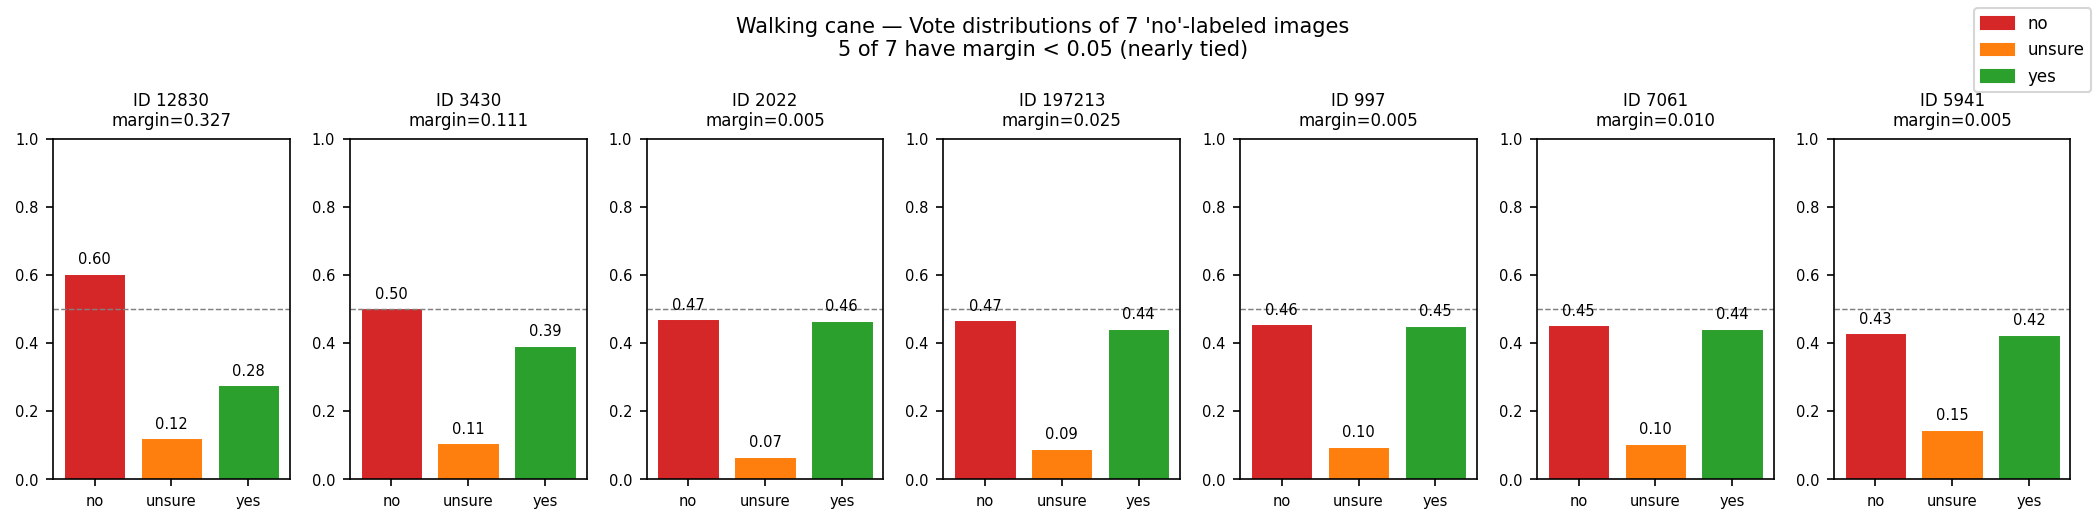
\includegraphics[width=0.95\linewidth]{images/walking_cane_votes.png}
\caption{\textbf{The seven majority-``no'' walking-cane images and their vote distributions.} IDs 2022, 197213, 997, 7061, and 5941 all have margin $<0.05$ between the top two classes (``no'' and ``yes''). Hard-CE training treats these as confident negatives and conflicts with the 45 confident positives in the rest of the cane distribution. Soft-KL retains the empirical bimodality and predicts $[\hat{p}_\mathrm{no} \approx 0.4,\, \hat{p}_\mathrm{unsure} \approx 0.1,\, \hat{p}_\mathrm{yes} \approx 0.5]$, the calibrated correct answer that explains the $+42\%$ relative F1 gain.}
\label{fig:cane_votes}
\end{figure}

\FloatBarrier
\section{Geographic Transfer: Per-City Detail}
\label{app:transfer}

This appendix expands the Geographic transfer probe paragraph in \S\ref{sec:results}. Figure~\ref{fig:generalization} shows the per-city balanced accuracy across Pittsburgh, Detroit, Zurich, and Taipei; Table~\ref{tab:supp_gen} reports the underlying counts, baselines, and gains.

\begin{figure}[!ht]
\centering
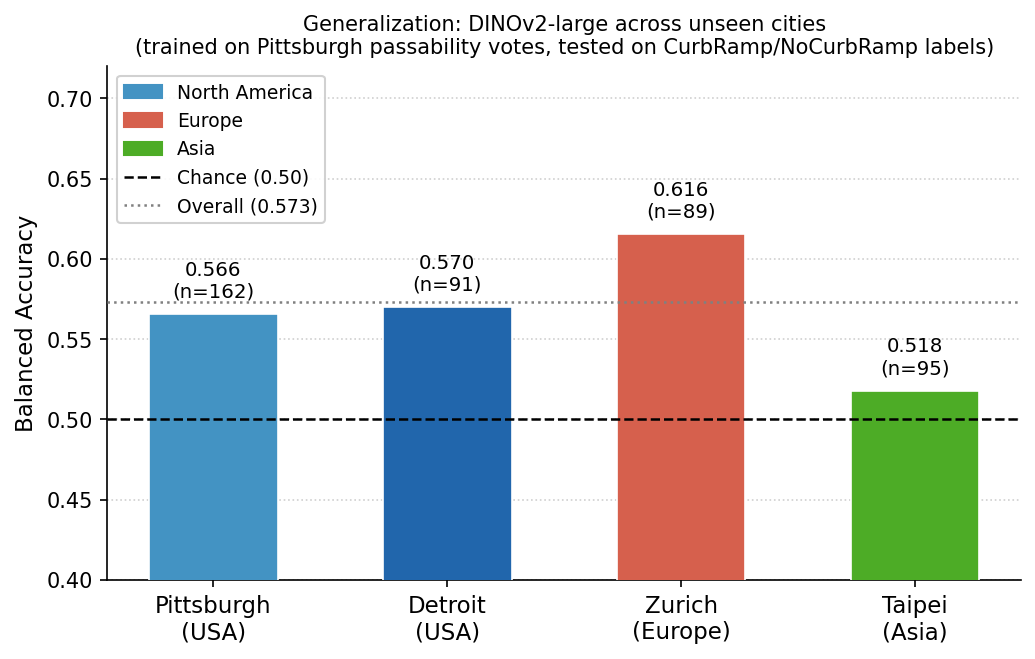
\includegraphics[width=0.80\linewidth]{images/generalization_figure.png}
\caption{Per-city balanced accuracy for DINOv2-large + Soft-KL on binary CurbRamp labels in unseen cities. Dashed line = chance ($0.50$). Pittsburgh/Detroit consistency rules out city-specific overfitting; Zurich gains $+11.6$\,pp (Amsterdam in training); Taipei is only $+1.8$\,pp above chance, the Western-centric-data limit.}
\label{fig:generalization}
\end{figure}

\begin{table}[!ht]
\caption{\textbf{Per-city generalization details.} DINOv2-large + Soft-KL trained on the 52-view passability benchmark, evaluated on Project Sidewalk binary CurbRamp labels in each city. ``Maj.'' = always-predict-majority-class baseline.}
\label{tab:supp_gen}
\centering\scriptsize
\setlength{\tabcolsep}{3.5pt}
\begin{tabular}{@{}llccccc@{}}
\toprule
\textbf{City} & \textbf{Region} & $n$ & \textbf{Bal.Acc} & \textbf{Maj.} & \textbf{Gain (pp)} & \textbf{Notes} \\
\midrule
Pittsburgh & N.America & 162 & 0.566 & 0.500 & $+6.6$ & in-distribution \\
Detroit    & N.America & 91  & 0.570 & 0.500 & $+7.0$ & similar Midwest US \\
Zurich     & Europe    & 89  & 0.616 & 0.500 & $+11.6$ & strong transfer \\
Taipei     & Asia      & 95  & 0.518 & 0.500 & $+1.8$ & near-chance \\
\midrule
\textbf{All} & n/a & \textbf{437} & \textbf{0.573} & 0.500 & $+7.3$ & weighted mean \\
\bottomrule
\end{tabular}
\end{table}

\FloatBarrier
\section{Routing: Pareto Analysis}
\label{app:pareto}

This appendix supports two routing claims in \S\ref{sec:routing}: (i) the choice $\beta_c{=}8$ and (ii) the Monte Carlo distributional behaviour. Table~\ref{tab:supp_pareto} and Fig.~\ref{fig:supp_pareto} give the per-aid Pareto sweep over $\beta_c \in \{1,2,4,8,16\}$; the inflection between $\beta_c=4$ and $\beta_c=8$ produces the largest accessibility gain per unit of distance overhead. Table~\ref{tab:supp_mc_full} and Figs.~\ref{fig:supp_mc_box},~\ref{fig:mc_pareto} report the full P25/P50/P75 distribution of the $10{,}000$-pair Monte Carlo evaluation; distance overhead is right-skewed (median $<1\%$ for all aids, while the mean is $4$--$5\%$).

\begin{table}[!ht]
\caption{\textbf{Barrier-cost sweep on the canonical OD pair.} Each cell shows ($\Delta\bar{p}_\mathrm{yes}$, $\Delta\ell$ \%). Bold marks the chosen operating point.}
\label{tab:supp_pareto}
\centering\scriptsize
\setlength{\tabcolsep}{4pt}
\begin{tabular}{@{}lccccc@{}}
\toprule
$\beta_c$ & \textbf{Cane} & \textbf{Walker} & \textbf{Scooter} & \textbf{Man.WC} & \textbf{Mot.WC} \\
\midrule
 1 & (0.029, 0.6) & (0.000, 0.0) & (0.000, 0.0) & (0.000, 0.0) & (0.000, 0.0) \\
 2 & (0.029, 0.6) & (0.026, 0.6) & (0.000, 0.0) & (0.000, 0.0) & (0.000, 0.0) \\
 4 & (0.145, 17.8) & (0.144, 24.8) & (0.140, 17.8) & (0.130, 17.8) & (0.133, 17.8) \\
\textbf{8} & \textbf{(0.155, 24.8)} & \textbf{(0.144, 24.8)} & \textbf{(0.140, 17.8)} & \textbf{(0.134, 19.3)} & \textbf{(0.146, 24.8)} \\
16 & (0.155, 24.8) & (0.144, 24.8) & (0.146, 24.8) & (0.140, 24.8) & (0.146, 24.8) \\
\bottomrule
\end{tabular}
\end{table}

\begin{figure}[!ht]
\centering
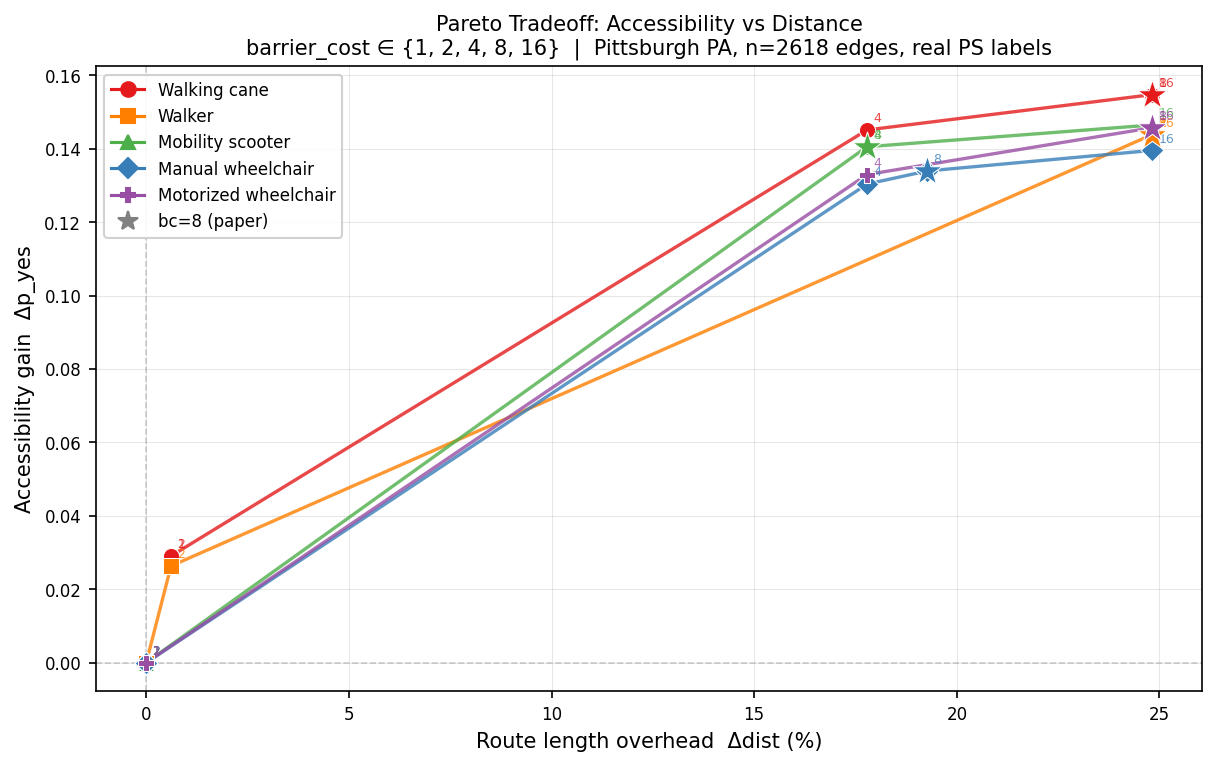
\includegraphics[width=0.80\linewidth]{images/pareto_barrier_cost.png}
\caption{Pareto curve for $\beta_c \in \{1,2,4,8,16\}$, averaged across the five mobility aids. The accessibility gain saturates past $\beta_c=8$, justifying our operating point.}
\label{fig:supp_pareto}
\end{figure}

\begin{table}[!ht]
\caption{\textbf{Full Monte Carlo distribution ($10{,}000$ OD pairs).} P25, P50, P75 of $\Delta\bar{p}_\mathrm{yes}$ and $\Delta\ell\%$, plus the fraction of pairs improved. Pittsburgh OSM graph, $\beta_c=8$, seed = 42, min separation 200~m.}
\label{tab:supp_mc_full}
\centering\scriptsize
\setlength{\tabcolsep}{3pt}
\begin{tabular}{@{}lccccccccc@{}}
\toprule
\textbf{Aid} & \multicolumn{3}{c}{$\Delta\bar{p}_\mathrm{yes}$} & \multicolumn{3}{c}{$\Delta\ell\,\%$} & \textbf{\% impr.} & $\bar{p}_\mathrm{yes}^\mathrm{std}$ & $\bar{p}_\mathrm{yes}^\mathrm{acc}$ \\
\cmidrule(lr){2-4} \cmidrule(lr){5-7}
& P25 & P50 & P75 & P25 & P50 & P75 & & & \\
\midrule
Walking cane         & 0.000 & 0.021 & 0.072 & 0.0 & 0.77 & n/a & 60.6 & 0.705 & 0.748 \\
Walker               & 0.000 & 0.020 & 0.085 & 0.0 & 0.39 & n/a & 59.2 & 0.625 & 0.673 \\
Mobility scooter     & 0.000 & 0.027 & 0.094 & 0.0 & 0.48 & n/a & 60.0 & 0.570 & 0.623 \\
Manual wheelchair    & 0.000 & 0.030 & 0.104 & 0.0 & 0.69 & n/a & 60.5 & 0.499 & 0.558 \\
Motorized wheelchair & 0.000 & 0.028 & 0.102 & 0.0 & 0.85 & n/a & 61.5 & 0.529 & 0.587 \\
\bottomrule
\end{tabular}
\end{table}

\begin{figure}[!ht]
\centering
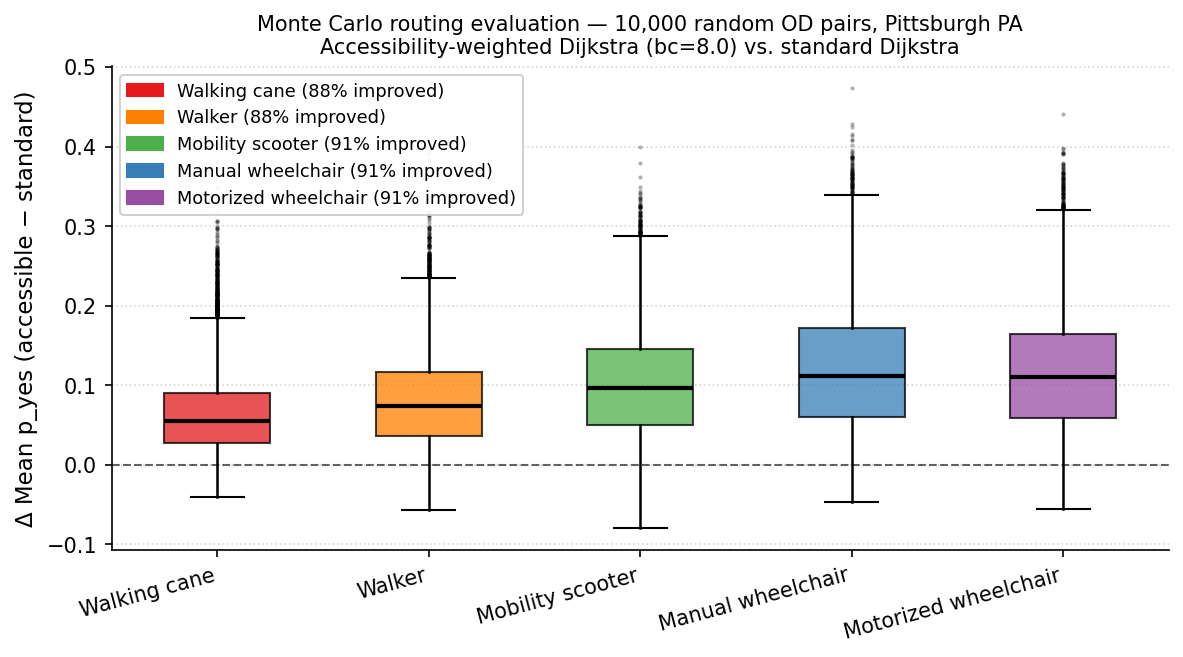
\includegraphics[width=0.80\linewidth]{images/monte_carlo_boxplot.png}
\caption{Boxplot of per-aid $\Delta\bar{p}_\mathrm{yes}$ on $10{,}000$ random OD pairs. All five aids show positive median improvement; the IQR confirms the rerouting benefit is widespread, not driven by outliers.}
\label{fig:supp_mc_box}
\end{figure}

\begin{figure}[!ht]
\centering
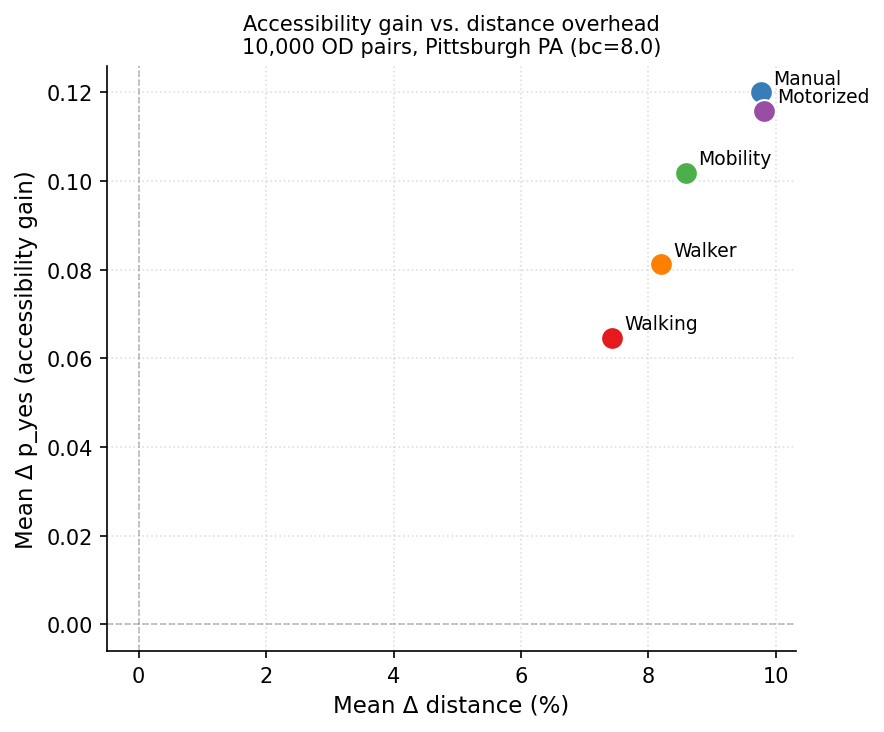
\includegraphics[width=0.80\linewidth]{images/monte_carlo_pareto.png}
\caption{Pareto scatter: mean accessibility gain $\Delta\bar{p}_\mathrm{yes}$ vs.\ mean distance overhead across $10{,}000$ random OD pairs. All five aids achieve positive accessibility gain at $7$--$10\%$ extra distance, confirming the routing benefit extends well beyond curated examples.}
\label{fig:mc_pareto}
\end{figure}

\FloatBarrier
\section{Routing: Per-Aid Visualisations and Comparisons}
\label{app:routing_viz}

This appendix supports the routing claims in \S\ref{sec:routing} with three pieces of evidence: (i) per-aid optimal paths for the canonical OD pair (Fig.~\ref{fig:supp_routes_grid}, Fig.~\ref{fig:routing_summary}); (ii) the full Std/ORS/Ours per-aid breakdown for the 40 routable Pittsburgh pairs (Table~\ref{tab:supp_ors_full}); and (iii) the Hard-CE vs Soft-KL routing cross-evaluation on the canonical OD pair (Table~\ref{tab:supp_crosseval}, Fig.~\ref{fig:hardce_comparison}).

\begin{figure}[!ht]
\centering
\begin{subfigure}[t]{0.32\linewidth}
\centering\vspace{0pt}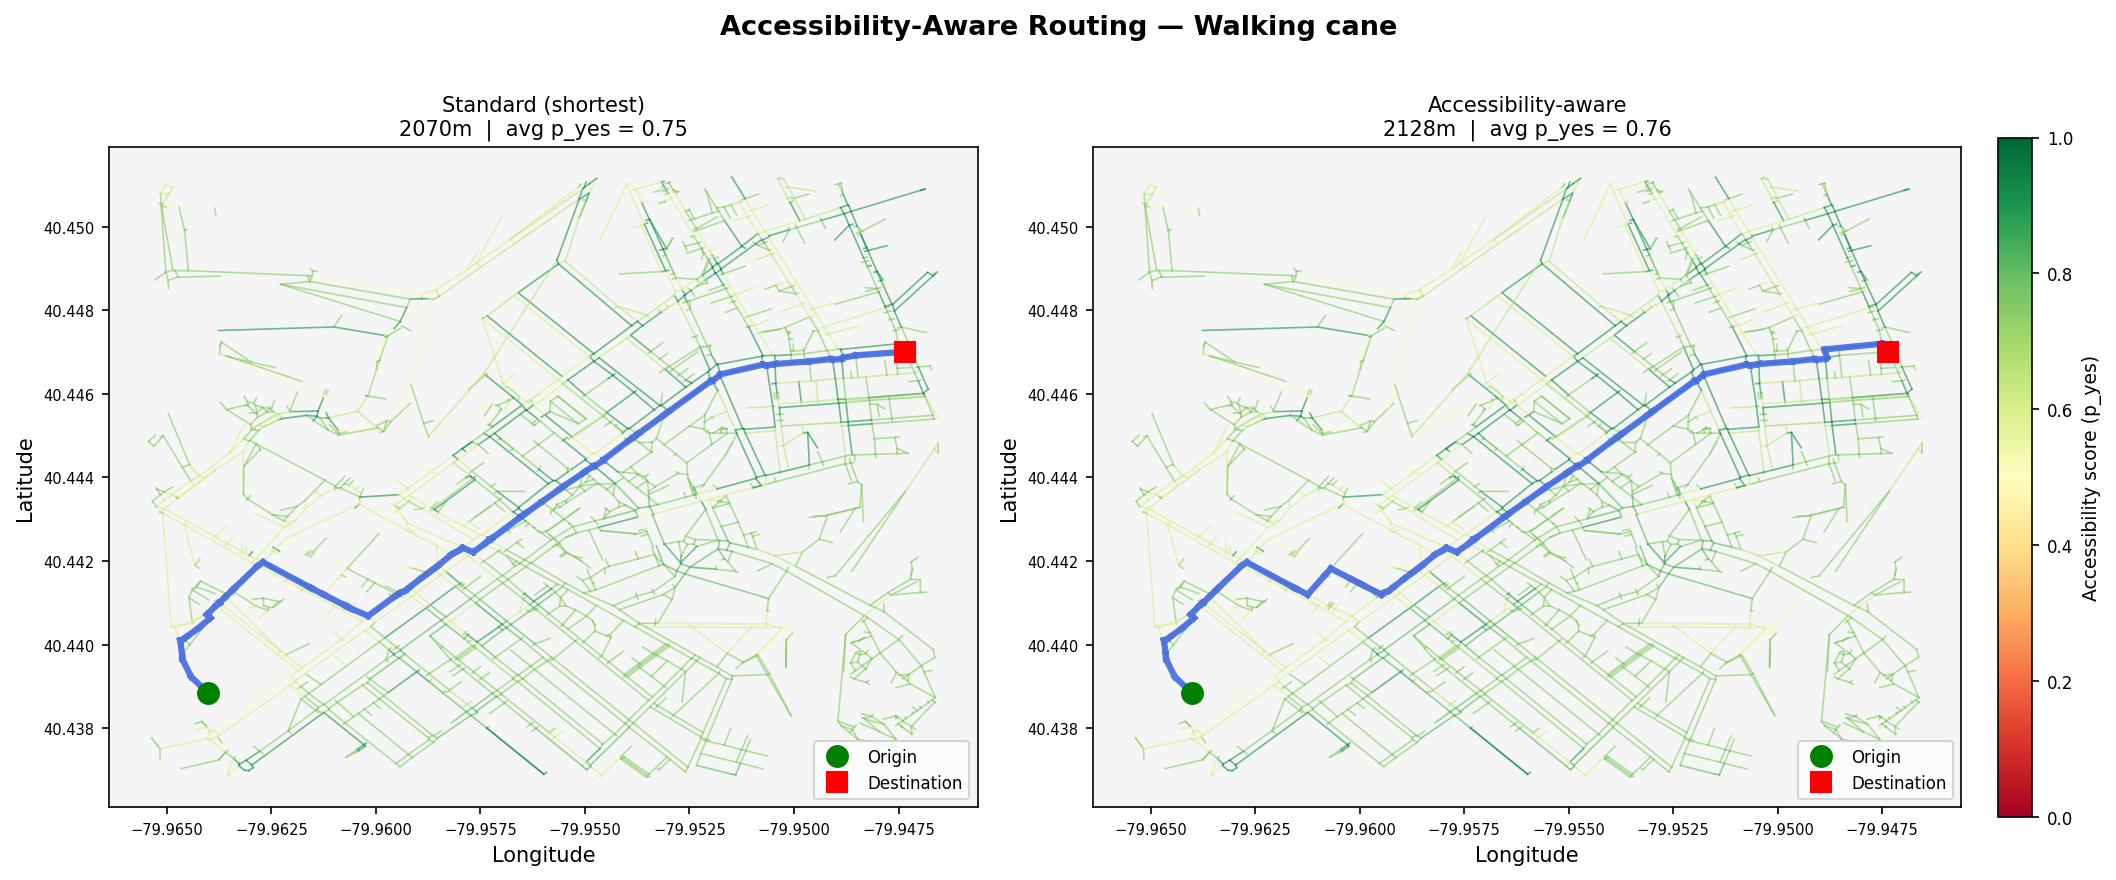
\includegraphics[width=\linewidth]{images/route_walking_cane.png}
\caption{Walking cane: $\bar{p}_\mathrm{yes} = 0.76$, $+2.8\%$ dist.}
\end{subfigure}
\hfill
\begin{subfigure}[t]{0.32\linewidth}
\centering\vspace{0pt}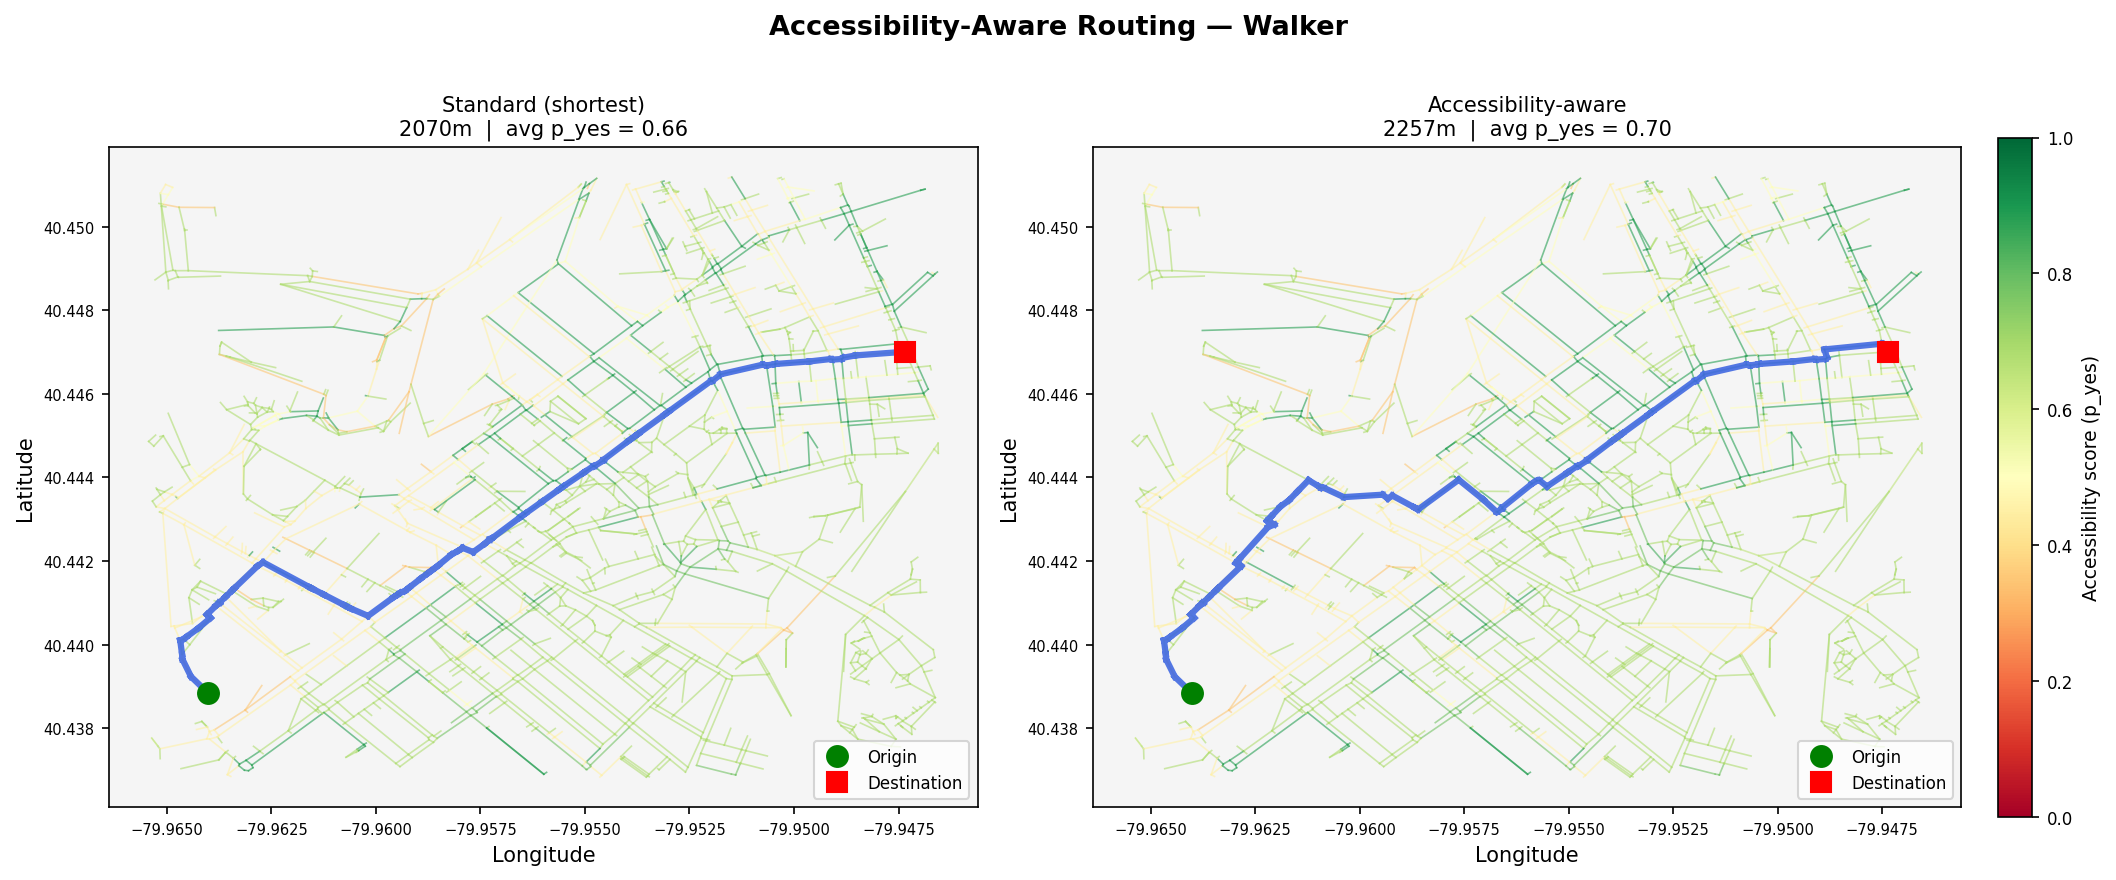
\includegraphics[width=\linewidth]{images/route_walker.png}
\caption{Walker: $\bar{p}_\mathrm{yes} = 0.70$, $+9.0\%$ dist.}
\end{subfigure}
\hfill
\begin{subfigure}[t]{0.32\linewidth}
\centering\vspace{0pt}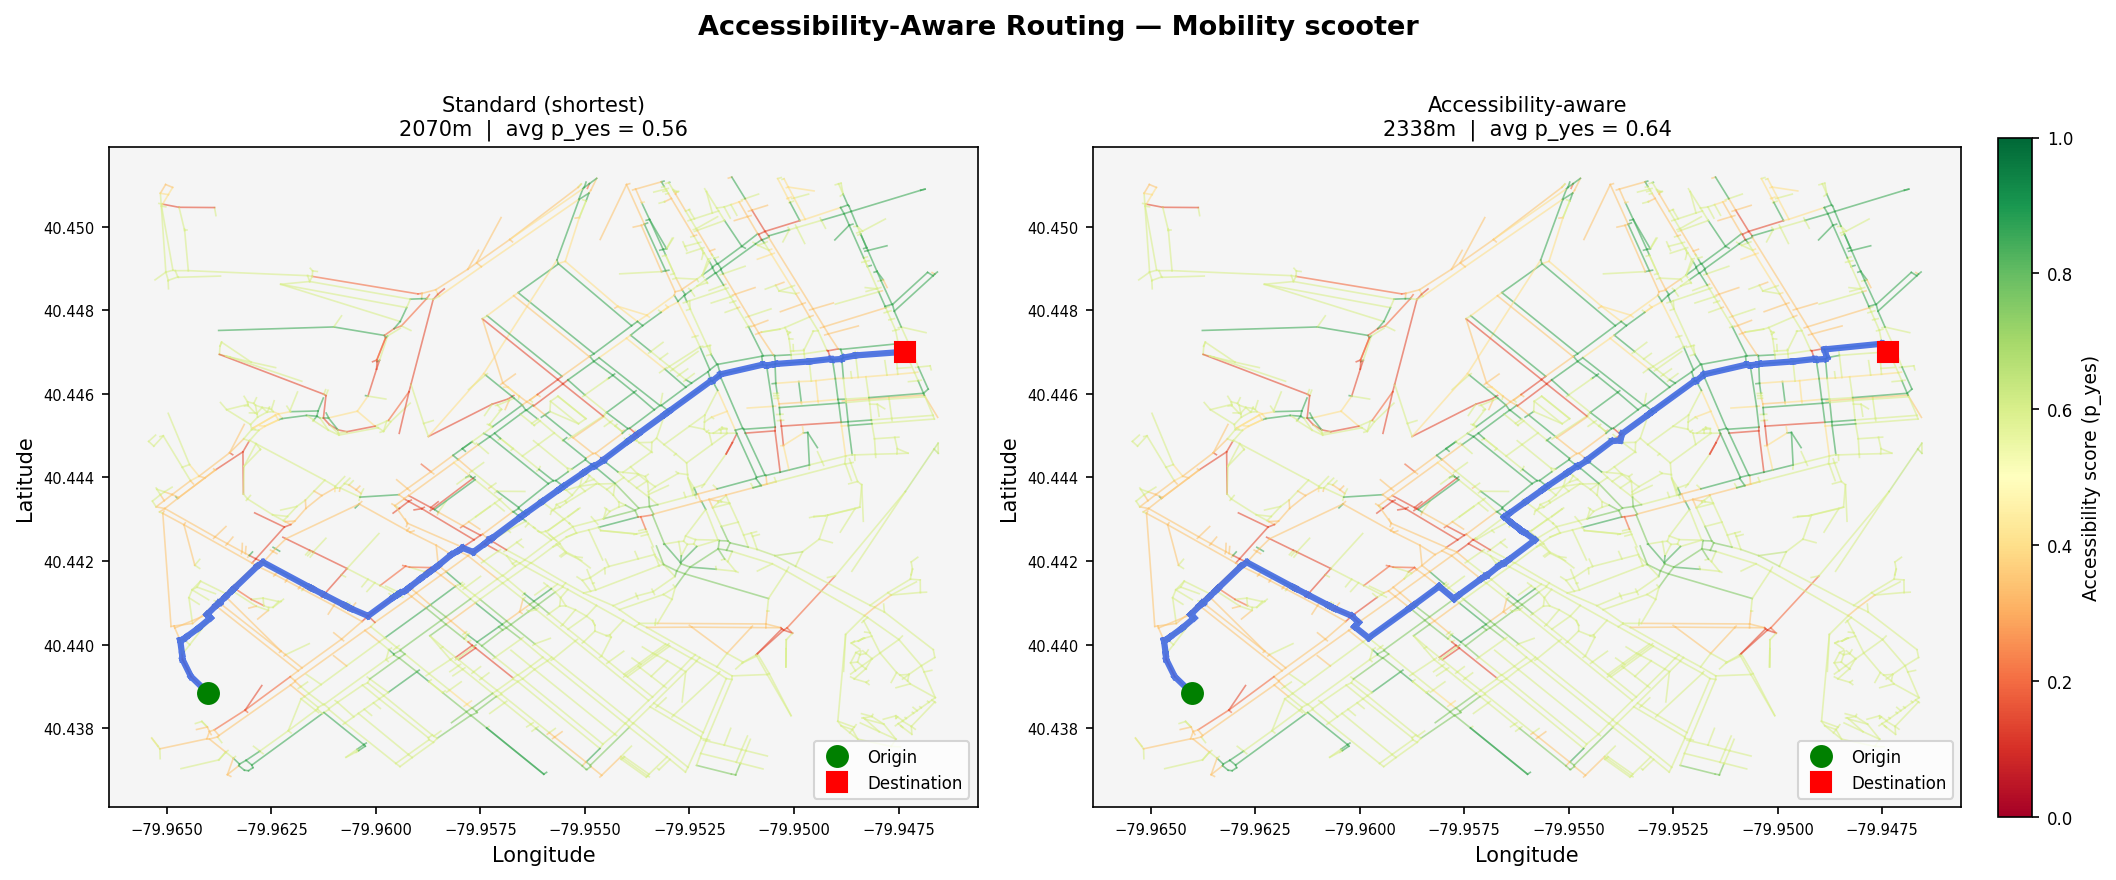
\includegraphics[width=\linewidth]{images/route_mobility_scooter.png}
\caption{Mobility scooter: $\bar{p}_\mathrm{yes} = 0.64$, $+12.9\%$ dist.}
\end{subfigure}\\[0.5em]
\begin{subfigure}[t]{0.32\linewidth}
\centering\vspace{0pt}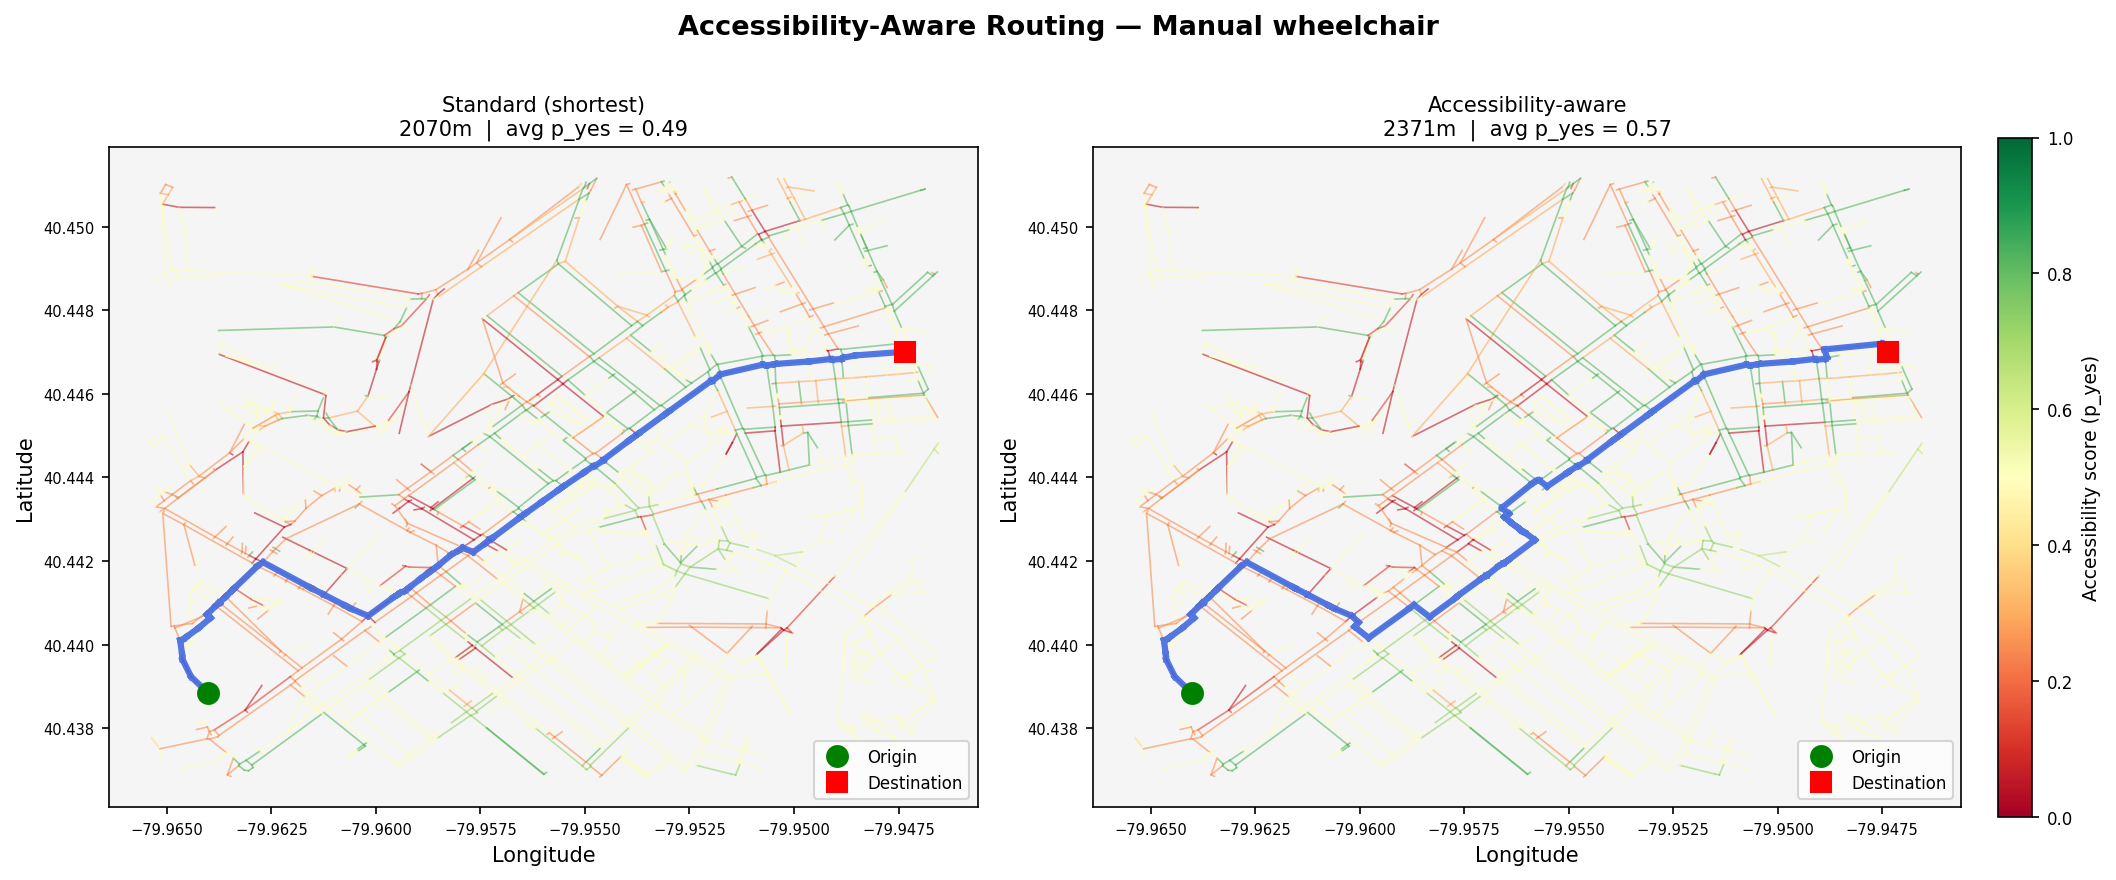
\includegraphics[width=\linewidth]{images/route_manual_wheelchair.png}
\caption{Manual wheelchair: $\bar{p}_\mathrm{yes} = 0.57$, $+14.5\%$ dist.}
\end{subfigure}
\hfill
\begin{subfigure}[t]{0.32\linewidth}
\centering\vspace{0pt}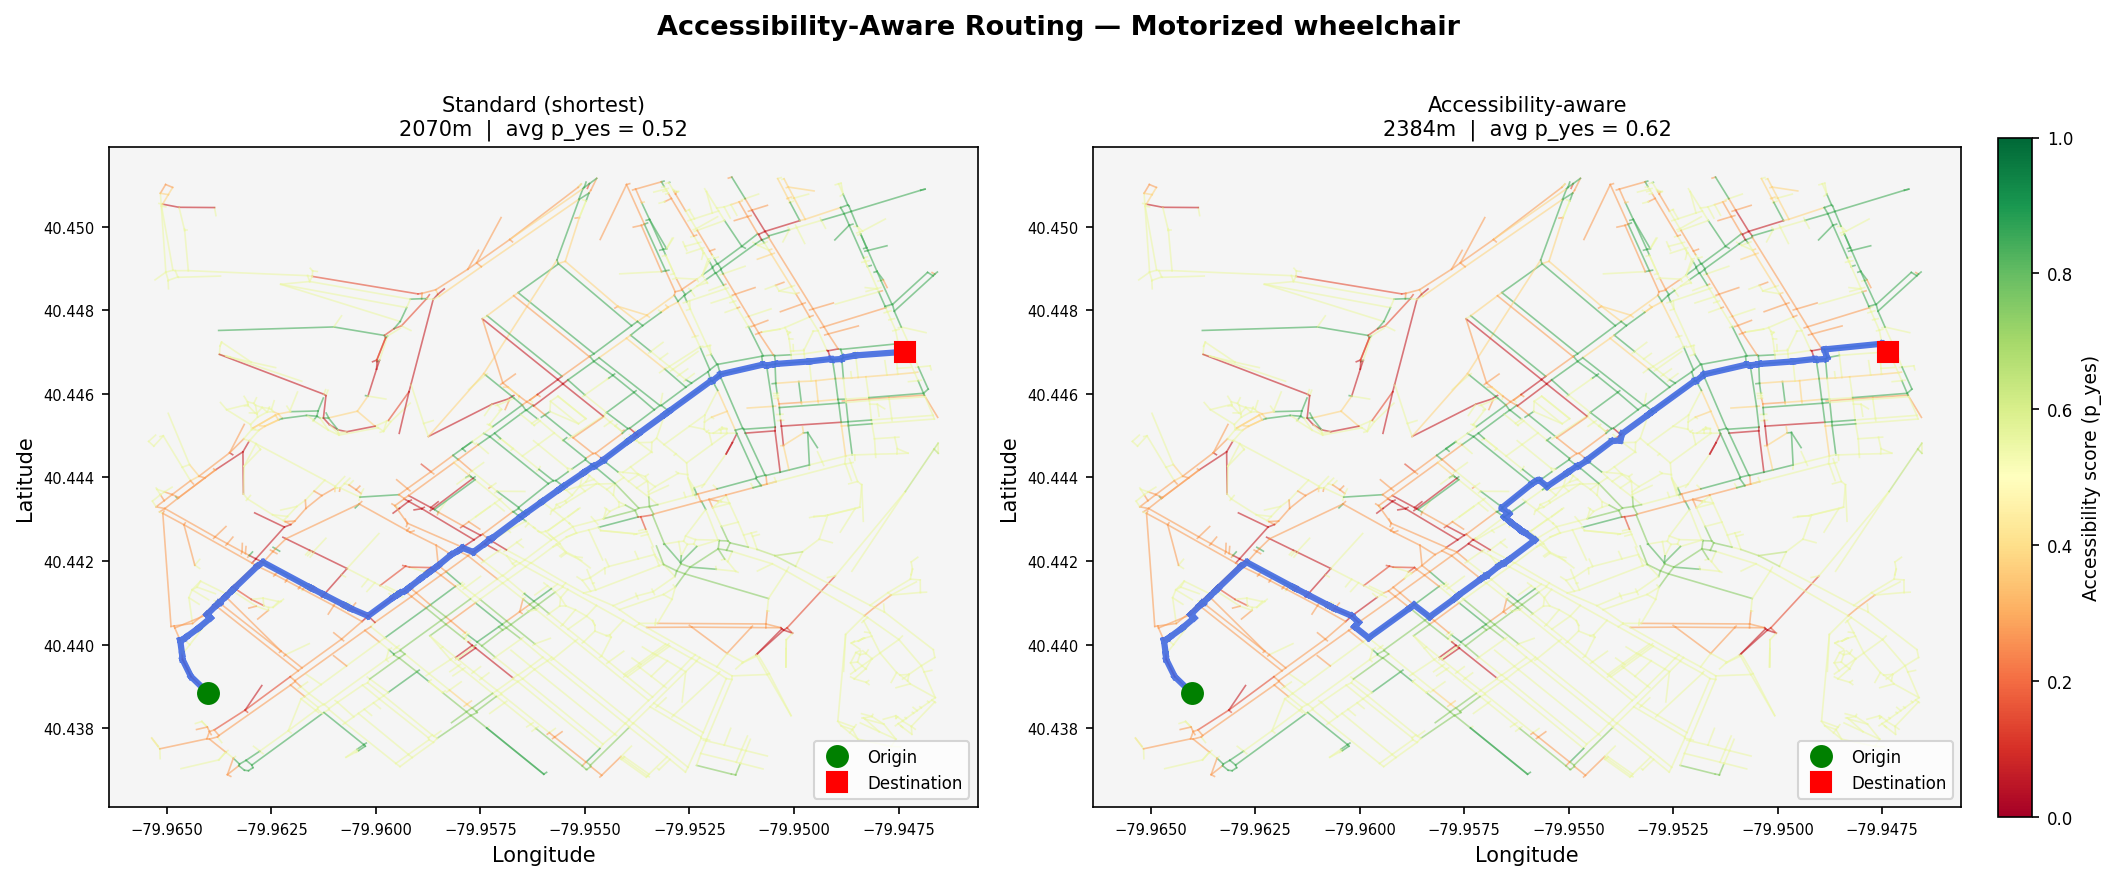
\includegraphics[width=\linewidth]{images/route_motorized_wheelchair.png}
\caption{Motorized wheelchair: $\bar{p}_\mathrm{yes} = 0.62$, $+15.1\%$ dist.}
\end{subfigure}
\caption{\textbf{Per-aid accessible routes (canonical OD pair, $\beta_c=8$).} The five panels reveal that the optimal accessible path is aid-specific: walking-cane and walker (top, easier aids) take the most efficient detour; manual and motorized wheelchairs (bottom) prefer further-removed but smoother corridors.}
\label{fig:supp_routes_grid}
\end{figure}

\begin{figure}[!ht]
\centering
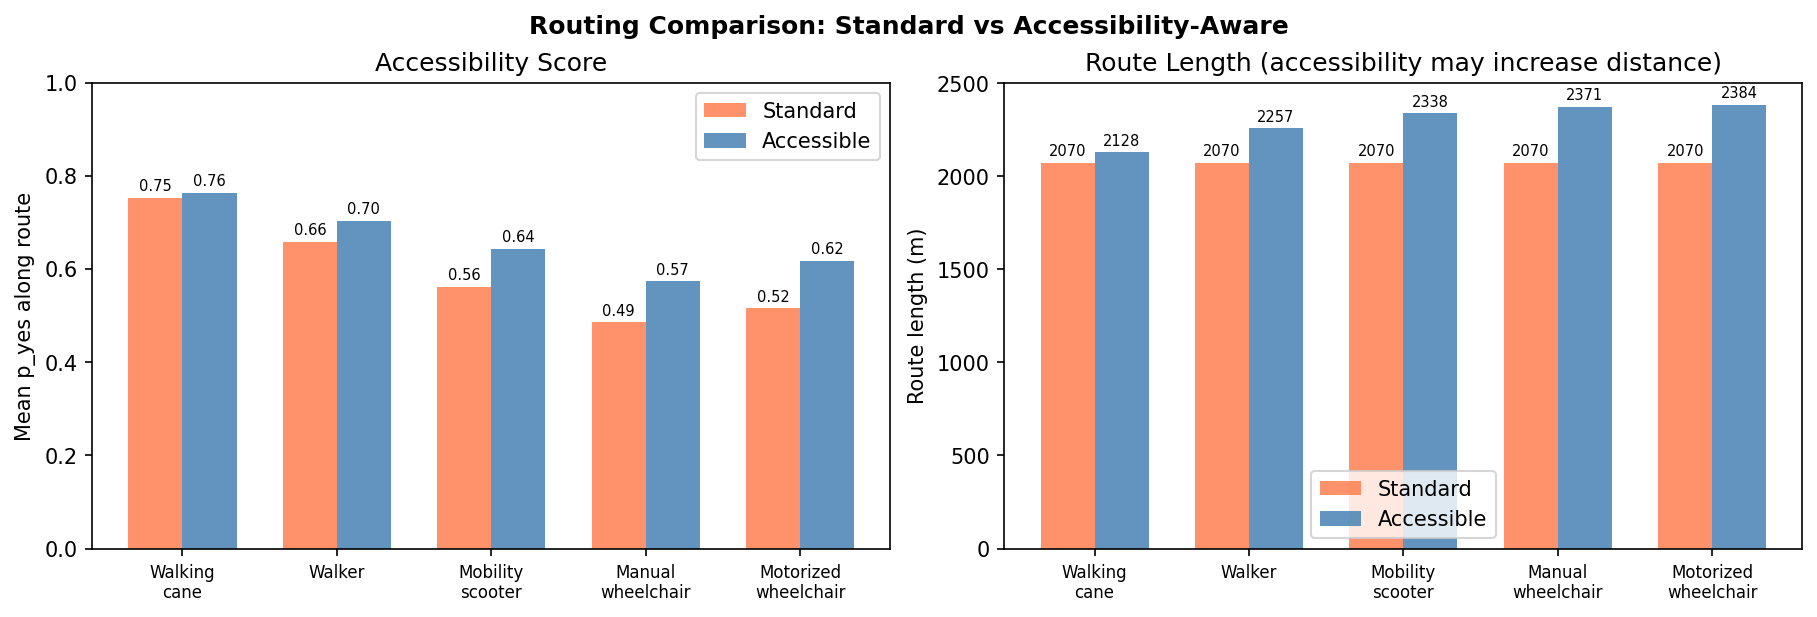
\includegraphics[width=0.80\linewidth]{images/routing_summary.png}
\caption{Per-aid summary for the canonical OD pair: accessibility score (left) and total route length (right). Walking cane (already $0.75$ baseline) gains the least in absolute $\hat{p}_\mathrm{yes}$ but the most in routing stability; the wheelchair aids gain $+0.07$ to $+0.13$ at $+12$ to $+18\%$ distance.}
\label{fig:routing_summary}
\end{figure}

\begin{table}[!ht]
\caption{\textbf{ORS wheelchair-profile comparison (full breakdown).} 40 routable OD pairs out of 50. ``ORS$-$Std.'' = gain ORS achieves over plain Dijkstra; ``Ours$-$ORS'' = our additional gain on top of ORS. Our method yields higher mean $\hat{p}_\mathrm{yes}$ than ORS on every aid in this Pittsburgh snapshot by $0.034$ to $0.047$. We queried the public OpenRouteService API \texttt{/v2/directions/wheelchair} endpoint between 2026-05-12 and 2026-05-14; the 10 unroutable pairs returned HTTP 400 with \texttt{``Could not find routable point within radius.''}}
\label{tab:supp_ors_full}
\centering\scriptsize
\setlength{\tabcolsep}{3.5pt}
\begin{tabular}{@{}lccccc@{}}
\toprule
\textbf{Aid} & \textbf{Std.} & \textbf{ORS} & \textbf{Ours} & \textbf{ORS$-$Std.} & \textbf{Ours$-$ORS} \\
\midrule
Walking cane         & 0.704 & 0.712 & 0.748 & $+0.009$ & $\mathbf{+0.036}$ \\
Walker               & 0.623 & 0.634 & 0.668 & $+0.011$ & $\mathbf{+0.034}$ \\
Mobility scooter     & 0.573 & 0.585 & 0.625 & $+0.012$ & $\mathbf{+0.040}$ \\
Manual wheelchair    & 0.505 & 0.519 & 0.566 & $+0.013$ & $\mathbf{+0.047}$ \\
Motorized wheelchair & 0.532 & 0.545 & 0.590 & $+0.013$ & $\mathbf{+0.045}$ \\
\midrule
\textit{Mean}        & 0.587 & 0.599 & 0.639 & $+0.012$ & $\mathbf{+0.040}$ \\
\bottomrule
\end{tabular}
\end{table}

\begin{table}[!ht]
\caption{\textbf{Hard-CE vs Soft-KL routing cross-evaluation on the canonical OD pair.} All $\hat{p}_\mathrm{yes}$ values evaluated by the calibrated Soft-KL metric (our reference risk estimate), except the last column which shows Hard-CE's own (inflated) self-assessment. Gap = Soft-KL route minus Hard-CE route by the calibrated metric. Hard-CE routes are 430--436~m vs.\ 412--575~m for Soft-KL; despite being shorter, they are consistently less accessible.}
\label{tab:supp_crosseval}
\centering\small
\setlength{\tabcolsep}{4pt}
\resizebox{\columnwidth}{!}{%
\begin{tabular}{@{}lcccccc@{}}
\toprule
\textbf{Aid} & \textbf{Std} & \textbf{SKL} & \textbf{HCE} & \textbf{Gap} & \textbf{HCE} & \textbf{HCE} \\
             & \textbf{(calibrated)} & \textbf{route} & \textbf{route} & \textbf{(SKL$-$HCE)} & \textbf{self-report} & \textbf{overestimate} \\
\midrule
Walking cane         & 0.516 & 0.671 & 0.657 & $+0.014$ & 0.721 & $+0.064$ \\
Walker               & 0.486 & 0.630 & 0.600 & $+0.030$ & 0.684 & $+0.085$ \\
Mobility scooter     & 0.459 & 0.600 & 0.587 & $+0.013$ & 0.675 & $+0.089$ \\
Manual wheelchair    & 0.442 & 0.576 & 0.561 & $+0.015$ & 0.660 & $+0.099$ \\
Motorized wheelchair & 0.446 & 0.592 & 0.572 & $+0.020$ & 0.625 & $+0.053$ \\
\bottomrule
\end{tabular}%
}
\end{table}

\begin{figure}[!ht]
\centering
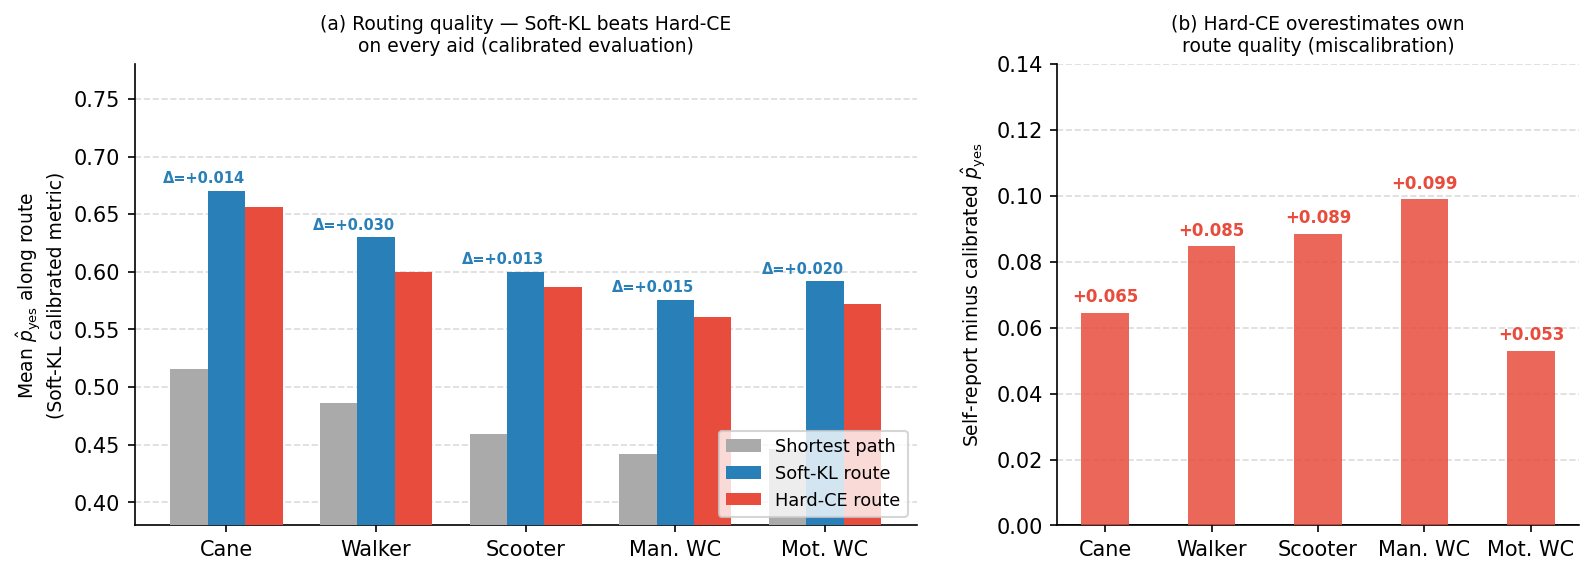
\includegraphics[width=0.80\linewidth]{images/routing_hardce_comparison.png}
\caption{Cross-evaluation of routing under Soft-KL vs.\ Hard-CE edge scores on the canonical Pittsburgh OD pair. Bars show mean $\hat{p}_\mathrm{yes}$ along each route, evaluated by the calibrated Soft-KL metric. Hard-CE routes (solid red) are uniformly lower-scoring than Soft-KL routes (blue) on the calibrated metric, despite Hard-CE's own inflated self-report (hatched red).}
\label{fig:hardce_comparison}
\end{figure}

\FloatBarrier
\section{Routing: Independent PS-Label Severity Validation}
\label{app:ps_val}

This appendix supports the independent-validation note in \S\ref{sec:limitations}.
We correlate model-predicted passability with Project Sidewalk (PS) label severity ($1$--$5$ scale, higher = worse) at the graph-edge level.
For each of the $420$ edges with at least one PS negative label (Obstacle, SurfaceProblem, NoCurbRamp, NoSidewalk) within $50$\,m, we compute the Spearman rank correlation between the edge's $\hat{p}_\mathrm{yes}$ and $-\overline{\mathrm{sev}}$ (negated so positive = good).
Severity scores were \emph{never} used in training or routing; only label \emph{types} entered the edge-scoring lookup for $40.4\%$ of edges, making severity an orthogonal signal.

\begin{table}[!ht]
\caption{\textbf{Edge-level Spearman correlation: $\hat{p}_\mathrm{yes}$ vs.\ $-$PS severity ($n$ edges with $\geq1$ nearby label, snap $50$\,m).} ``Inference'' edges are scored by DINOv2-large and are fully independent of PS data. Positive $r$ means higher predicted passability associates with lower severity. $p$-values two-tailed.}
\label{tab:ps_val}
\centering\scriptsize
\setlength{\tabcolsep}{5pt}
\begin{tabular}{@{}lcccc@{}}
\toprule
\textbf{Aid} & \textbf{Source} & $n$ & $r$ & $p$ \\
\midrule
\multirow{2}{*}{Walking cane}       & Inference (indep.) & 188 & $+0.247$ & $0.0006$ \\
                                     & All edges          & 420 & $+0.161$ & $0.0009$ \\
\midrule
\multirow{2}{*}{Manual wheelchair}  & Inference (indep.) & 188 & $+0.232$ & $0.0013$ \\
                                     & All edges          & 420 & $+0.123$ & $0.0118$ \\
\bottomrule
\end{tabular}
\end{table}

\noindent The significant positive correlation on inference-only edges confirms that the model's passability estimates are calibrated against an independent human-annotated accessibility measure, supporting the validity of the routing objective beyond its own circular metric.

\FloatBarrier
\section{Algorithms and Reproducibility}
\label{app:algo}

This appendix gives pseudocode for the two algorithms underlying the paper and the compute/reproducibility details required to replicate every number in the main text.

\subsection{Soft-KL Probe Training}

\begin{algorithm}[!ht]
\caption{Soft-KL training of a per-aid linear probe}
\label{alg:softkl}
\begin{algorithmic}[1]
\REQUIRE Frozen encoder $E$, training images $\{x_i\}_{i=1}^N$, vote distributions $\{\mathbf{y}_{i,a}\}$ for $a \in \mathrm{Aids}$
\STATE Pre-compute $\mathbf{f}_i = E(x_i)/\|E(x_i)\|_2$ once per image
\STATE Initialise $W_a, b_a$ from $\mathcal{N}(0, 0.01)$ for each aid $a$
\FOR{epoch $= 1$ to 50}
   \FOR{mini-batch $\mathcal{B} \subset \{1,\dots,N\}$ of size 64}
      \STATE $\hat{\mathbf{y}}_{i,a} = \mathrm{softmax}(W_a \mathbf{f}_i + b_a)$
      \STATE $w_{i,a} = 1 - H(\mathbf{y}_{i,a})/\hmax$
      \STATE $\mathcal{L} = \sum_{i \in \mathcal{B}}\sum_a w_{i,a} \kl(\mathbf{y}_{i,a}\|\hat{\mathbf{y}}_{i,a})$
      \STATE Update $\{W_a, b_a\}$ via AdamW (lr $10^{-3}$, wd $10^{-4}$)
   \ENDFOR
\ENDFOR
\RETURN $\{W_a, b_a\}_{a \in \mathrm{Aids}}$
\end{algorithmic}
\end{algorithm}

\subsection{Accessibility-Aware Dijkstra}

\begin{algorithm}[!ht]
\caption{Per-aid accessibility-aware shortest path}
\label{alg:dijkstra}
\begin{algorithmic}[1]
\REQUIRE Pedestrian graph $G=(V,E)$, edge lengths $\ell_e$, per-aid per-edge probabilities $\hat{p}^a_{\mathrm{yes},e}$, origin $s$, destination $t$, aid $a$, barrier cost $\beta_c$
\FOR{$e \in E$}
   \STATE $w_e^a \gets \ell_e \cdot (1 + \beta_c \,(1 - \hat{p}^a_{\mathrm{yes},e}))$
\ENDFOR
\STATE $P \gets$ Dijkstra$(G, s, t, w^a)$
\STATE $\bar{p}^a_{\mathrm{yes}}(P) \gets \frac{\sum_{e \in P} \ell_e \,\hat{p}^a_{\mathrm{yes},e}}{\sum_{e \in P} \ell_e}$
\RETURN $P$, $\bar{p}^a_{\mathrm{yes}}(P)$, $\sum_{e \in P} \ell_e$
\end{algorithmic}
\end{algorithm}

\subsection{Compute and Reproducibility}

\textbf{Hardware.} All experiments were run on a single NVIDIA A100 40~GB GPU. Encoder feature extraction for all 200 verified image crops takes 4 to 10\,s per encoder (DINOv2-large is the slowest at 9.8\,s). Soft-KL or Hard-CE probe training for the full 5-fold CV across one encoder takes 30 to 90\,s. The full 8-encoder $\times$ 2-loss CV grid runs end-to-end in $<30$ minutes.

\textbf{Software.} Python 3.9, PyTorch 2.2, transformers 4.40, timm 0.9.16, NetworkX 3.2, OSMnx 1.9. The OpenRouteService queries used the public API at \url{https://api.openrouteservice.org/v2/directions/wheelchair} on 2026-05-12 through 2026-05-14. Polyline decoding uses the \texttt{polyline} pip package v2.0.

\textbf{Random seeds.} All experiments use the same global seed (42) for NumPy, PyTorch (CPU + CUDA), Python \texttt{random}, and the panorama-level fold split. The Monte Carlo OD-pair sampler reseeds NumPy with the same seed before generating its 10{,}000 pairs.

\textbf{Code availability.} Code and pre-extracted features will be released on acceptance under an MIT licence, including: (i) the per-encoder feature extraction pipeline; (ii) Soft-KL / Hard-CE probe training; (iii) the accessibility-aware Dijkstra implementation; (iv) the ORS comparison harness; (v) the Monte Carlo evaluation; and (vi) all figure-generation notebooks.

\end{document}
